% addtional
\UseRawInputEncoding

%gibt an: Papierformat, Schriftgröße
\documentclass[a4paper,english,12pt]{article}
\setlength{\parskip}{0.2cm}
\setlength{\parindent}{0cm}
%-----------------------------------------------------------------------------------------------------------------------------
%Übersetzung von E in D
\usepackage[english]{babel} %changed to English
%Einstellung der Randabstände
\usepackage[lmargin={3.5cm},rmargin={2.5cm},tmargin={2.5cm},bmargin={2cm}]{geometry}
%zur Einbindung von Graphiken
\usepackage{graphicx}
%Bearbeitung von Kopf- und Fusszeile
\usepackage{fancyhdr}
%Schriftart
\usepackage{helvet}
%stellt unabhängige Textmarken zu Verfügung
\usepackage{extramarks}
%aktiviert eine Umgebung in der der Mathematikmodus aktiv ist
\usepackage{amsmath}
%aktiviert eine Umgebung in der der Mathematikmodus aktiv ist
\usepackage{amsthm}
%aktiviert eine Umgebung in der der Mathematikmodus aktiv ist
\usepackage{amssymb}
%aktiviert Hyperlinks
\usepackage{hyperref} 
%Stellt das Eurozeichen € zu Verfügung
\usepackage[right]{eurosym}
%Übersetzt die Tastatureingaben für LaTex
%\usepackage[latin1]{inputenc}                                                          <-- auskommentiert wegen Sonderzeichen etc (zusammen mit Zeile 1)
\usepackage{fancybox} 
\usepackage[dvipsnames]{xcolor} %more pre-defined colors
\usepackage{color}
\usepackage{colortbl} %colors in tables for horizontal and vertical lines
\definecolor{myorange}{RGB}{247,150,0} %colors from ppt graphics for uniform coloring
\definecolor{mygreen}{RGB}{0,150,130} %KIT green/blue
\definecolor{myred}{RGB}{192,80,77}
\definecolor{myblue}{RGB}{79,129,189}
\usepackage{float}
\usepackage{framed}
\usepackage{url}
\usepackage{verbatim} %multi-line comments
\usepackage[titles]{tocloft} %toc design

\usepackage{natbib}

\usepackage{booktabs}
\usepackage{tabularx} %Tabellen, die sich der Seitenbreite anpassen

\usepackage{multirow} % Verbundene Zellen in Tabellen
\usepackage{rotating} % Quergestellte Tabellen
\usepackage{rotfloat}

\usepackage[bottom]{footmisc} %Fußnoten immer am Ende der Seite
\usepackage{tikz} %for graphics, eg trees
\usepackage{tcolorbox} %color for graphics
\usepackage{pgfkeys}
\usepackage{multicol} %multi-column
\usepackage{colortbl} % colour of table lines
\usepackage{algorithm}
\usepackage{algpseudocode}
\usepackage{algorithmicx} %layout for algorithms
\usepackage{xfrac} %layout for fractions
%Definitionen
\newtheoremstyle{mystyle}% name
{10pt}% Space above
{10pt}% Space below
{\itshape}% Body font
{}% Indent amount: 
{\bfseries}% Theorem head font
{:}% Punctuation after theorem head
{0.5em}% Space after theorem head
{\thmname{#1}\thmnumber{ #2}:\thmnote{ #3}}% Theorem head 

\theoremstyle{mystyle}% default
\newtheorem{definition}{Definition}
\numberwithin{equation}{section}
\renewcommand{\proofname}{Beweis}


%Paragraphen

\newcommand{\myparagraph}[1]{\paragraph{}\mbox{}\\}


% ADDITIONAL PACKAGES

\usepackage{cleveref}

\usepackage{adjustbox}

\usepackage{makecell}
\usepackage{amssymb}% http://ctan.org/pkg/amssymb
\usepackage{pifont}% http://ctan.org/pkg/pifont

\newcommand{\cmark}{\ding{51}}%
\newcommand{\xmark}{\ding{55}}%

% ADDITIONAL PACKAGES

%-----------------------------------------------------------------------------------------------------------------------------------------
\renewcommand{\baselinestretch}{1.24}
\fancyhead[LO]{\slshape \small \firstleftmark}
\fancyhead[RO]{\normalsize\thepage} \fancyfoot{}
\begin{document}
%-----------------------------------------------------------------------------------------------------------------------------------------
%Titelseite
\begin{titlepage}
% font / Schriftart
%------------------	

	
	
\begin{figure}[htbp]
  %\centering
  
  \begin{minipage}[b]{.2\textwidth}
  %\begin{minipage}[b]{.4\textwidth}
    
\includegraphics[width=4cm]{0_Logos/kit.jpg}  
  \end{minipage}%
  \hfill
  \begin{minipage}[b]{.8\textwidth}
	\begin{flushright}
	    
\includegraphics[width=3cm]{0_Logos/IISM_logo.png}
	    \hspace{0.3cm}
        
\includegraphics[width=2.5cm]{0_Logos/KSRI_logo.png}  
        \hspace{0.3cm}
        
\includegraphics[width=2.5cm]{0_Logos/DKFZ_cropped.png}
	\end{flushright}
  \end{minipage}
  
\end{figure}

%\vspace*{1cm}
\vspace*{0.5cm}
\begin{center}
		%\Huge{Real-World Federated Learning for Medical Images: Requirements and Demonstrations}
		\Huge{Federated Learning on Medical Images: Closing Gaps to the Real-World}
		%\vspace*{1.5cm}\\
		\vspace*{1.0cm}\\
		\Large{Master Thesis}\\
		\Large{by}\\
		%\vspace*{1cm}
		\vspace*{0.5cm}
		\huge{Marius Kempf}\\
		\large{Matriculation number: 1843925}\\
		%\vspace*{1cm}
		\vspace*{0.5cm}
		\Large{
			At the Department of Economics and Management
			%\\ \vspace*{1cm}
			\\ \vspace*{0.75cm}
			Digital Service Innovation (DSI)
			\\ \vspace*{0.5cm}
			Karlsruhe Service Research Institute (KSRI) \& \\
			Institute of Information Systems and Marketing (IISM)
		}
	\end{center}
	%\vspace*{0.75cm}
	\vspace*{0.25cm}
\Large{
\begin{center}
\begin{tabular}[ht]{l c l}
  Advisor:          & \hfill    & Prof. Dr. Gerhard Satzger \\
  Second Advisor:   & \hfill    & Prof. Dr. Hansj\"org Fromm \\
  Advisor DKFZ:     & \hfill    & Prof. Dr. Klaus H. Maier-Hein \\
  Supervisor:       & \hfill    & Dr. Niklas K\"uhl \\
  Supervisors DKFZ  & \hfill    & Klaus Kades, Maximilian Zenk \\
 % \mbox{} & \hfill	&Name\\
  Date of Submission:  & \hfill & August 2, 2021 \\
\end{tabular}
\end{center}
}


\vspace*{1.0cm}
	\tiny{KIT -- The Research University in the Helmholtz Association} \hfill \small{\textbf{www.kit.edu} }
\end{titlepage}


\thispagestyle{empty}\cleardoublepage

\mbox{}\thispagestyle{empty}
\cleardoublepage

{\Large \textbf{Declaration of Academic Integrity}} 

\bigskip
I hereby confirm that the present thesis is solely my own work and that if any text passages or diagrams from books, papers, the Web or
other sources have been copied or in any other way used, all references---including those found in
electronic media---have been acknowledged and fully cited. \\



\vspace{1cm}
 
\textit{Karlsruhe, 02 August 2021} \hspace{4cm} \textit{Marius Kempf} \\


\thispagestyle{empty}\cleardoublepage

{\Large \textbf{Abstract}} 

\bigskip

Data science offers many opportunities to gain new and valuable insights from medical data to achieve enhanced patient care. The potential becomes even greater the more data can be analyzed and used to train machine learning models. In particular, for deep learning, numerous training samples are needed to achieve adequate performance and generalizability for the sensitive healthcare domain. However, medical data is highly sensitive and must therefore be treated very carefully for good reasons.
% question
Federated learning is a machine learning paradigm that allows to leverage geographically distributed data while maintaining privacy by sharing models instead of raw data during the training process.
The potential and performance of models trained federally have already been demonstrated, but real-world applications in the field of medical imaging are still rare. To bridge the gap between simulations and actual experiments across medical institutions, technical solutions are required.
Recently, a multitude of promising projects aiming to provide solutions for federated learning have emerged. However, they must fulfill specific requirements for a meaningful usage in a medical environment.
We, therefore, ask the question, what is needed to bring federated learning solutions into clinics and how a solution could look like.
% methodology
We compare existing solutions and demonstrate a combination of PySyft and the Joint Imaging Platform.
Further, a solution purely based on the Joint Imaging Platform, which is already installed at several German clinics, is introduced: JIP Federated. Its capability is demonstrated with a federated segmentation experiment on distributed brain MRI scans.
% results
Our results show the following.
The gap of a comprehensive solution fulfilling all requirements could be narrowed to some extent, but not yet closed---Additional effort is required.
Further, JIP Federated is a flexible solution that allows data scientists to freely implement their own algorithms, and is available as an open-source project. 
Together with the Joint Imaging Platform's features developed for medical imaging, JIP Federated offers a promising solution to apply federated learning across medical institutions, thus, allowing distributed analyses while preserving privacy.


\mbox{}\thispagestyle{empty}
\cleardoublepage
\rmfamily \pagestyle{fancy} \setcounter{secnumdepth}{4}


\pagenumbering{roman}
\setcounter{page}{4} 
\setlength\cftparskip{-5pt}
\setlength\cftbeforesecskip{-1pt}
\setlength\cftaftertoctitleskip{-10pt}
\tableofcontents
\cleardoublepage
\phantomsection
\addcontentsline{toc}{section}{Acronyms} %include in toc w/o numbering

\markboth{ACRONYMS}{Acronyms}
\section*{Acronyms}
\begin{table}[H]
    \begin{tabular}{p{4cm} p{10cm}}
     API    & Application Programming Interface \\
     AUROC  & Area Under the Receiver Operator Characteristic \\
     BraTS  & Brain Tumor Segmentation \\
     CNN    & Convolutional Neural Network \\
     CPU    & Central Processing Unit \\
     CV     & Computer Vision \\
     DAG    & Directed Acyclic Graph \\
     DC     & Dice Score \\
     DKTK   & German Cancer Consortium \\
     DL     & Deep Learning \\
     ET     & Enhancing Tumor \\
     FATE   & Federated AI Technology Enabler \\
     FedAvg & Federated Averaging \\
     FL     & Federated Learning \\
     FN     & False Negative \\
     FP     & False Positive \\
     FPR    & False Positive Rate \\
     GDPR   & General Data Protection Regulation \\
     GPU    & Graphical Processing Unit \\
     GUI    & Graphical User Interface \\
     HIPPA  & Health Insurance Portability and Accountability Act \\
     JIP    & Joint Imaging Platform \\
     ML     & Machine Learning \\
     MLP    & Multi Layer Perceptron \\
     MNIST  & Modified National Insitute of Standards and Technology \\
     MONAI  & Medical Open Network for AI \\
     MRI    & Magnetic Resonance Imaging \\
     PFL    & PaddleFL \\
     PP     & PaddlePaddle \\
     ROC    & Receiver Operator Characterisitc \\
     SGD    & Stochastic Gradient Descent \\
     SVM    & Support Vector Machine \\
     TC     & Tumor Core \\
     TFF    & TensorFlow Federated \\
     TN     & True Negative \\
     TP     & True Positive \\
     TPR    & True Positive Rate \\
     WT     & Whole Tumor
    \end{tabular}%
\end{table}%


\cleardoublepage
\phantomsection
\addcontentsline{toc}{section}{List of Figures} %include in toc w/o numbering
\listoffigures
\cleardoublepage
\phantomsection
\addcontentsline{toc}{section}{List of Tables} %include in toc w/o numbering
\listoftables
\cleardoublepage

\setcounter{page}{2} \pagenumbering{arabic}

\interfootnotelinepenalty=10000 % Keine Seitenumbrüche bei Fußnoten

 % % % % % % % % % % % % %INHALTE % % % % % % % % % % % % % %
 
 \section{Introduction}
\label{sec:Introduction}

% good old time
From the moment it was possible to load and store medical images into a computer, researchers have begun to develop solutions for automated image analysis.
Initially, analysis was done by, from today's perspective, simple rule-based systems.
Later on, also machine learning (ML) techniques were applied. For the first applications of machine learning, features were extracted manually. Sample data was collected, and \textit{handcrafted} feature vectors containing information about characteristics such as shapes, sizes or edges were derived from the images. 
Then, the features were entered as input to an ML model such as a multilayer perceptron (MLP) \citep{Rumelhart1986LearningErrors} or a support vector machine (SVM) \citep{Vapnik1995TheTheory}. During training, the models search for the most optimal decision boundary, which is then used to separate the classes (in case of a classification).

% machine learning with cnns
The next step was to leave it to the computers, respectively models, to decide what information they need from an image to serve as a good representation. The concept lets layered networks extract the features themselves by starting with high-level features and going down to very specific low-level features. To this day, the most successful type of such models for image analysis are convolutional neural networks (CNNs). The architectures contain a multitude of layers which transform their input by applying convolutional filters. This first part of the model can be referred to as \textit{feature-extractor}, because it generates meaningful features based on the given input by applying convolutions. It is followed by a classifier, using the extracted features for its decision-making. In contrast to previous approaches, convolutional neural networks are an end-to-end processing architecture using the raw input images. For computer vision (CV), convolutional neural networks are the technology of choice to this day.

Back in the year 1998, \cite{LeCun1998Gradient-basedRecognition} published first pioneering work using such CNNs in the real-world application of hand-written digit recognition.
Over time, convolutional neural networks were used for increasingly complex applications and thus the models became also more complex, having millions of trainable parameters.
This was only possible because the available computing resources and the available image data grew at the same.
% übergang zu deep learning
The size of the models and the architecture of consecutively stacked layers led to the term Deep Learning (DL) \citep{Lecun2015DeepLearning}.
A major breakthrough was the publication of \cite{Krizhevsky2012ImageNetNetworks} within the context of the ImageNet challenge\footnote{\url{https://www.image-net.org/index.php}} in 2012. The authors introduced a convolutional neural network referred to as AlexNet and won the challenge by a large margin.
Following this performance leap, related architectures were developed, that became even deeper.

The recent years have proved that deep learning is able to achieve state-of-the-art performance, even surpassing human-level performance, on a multitude of different tasks not only in computer vision but also in speech recognition and natural language processing \cite{HeDelvingClassification, Hinton2012DeepGroups, Devlin2019BERT:Understanding}. Also, within the medical domain, deep learning has gained attention, and models with expert-level performance have been reported \citep{Esteva2017Dermatologist-levelNetworks}.

% amount of data
The availability of huge amounts of annotated data is one of the key factors for this success, namely datasets such as ImageNet \cite{Deng2009ImageNet:Database}. Deep learning in the medical domain is not different in that regard: To achieve human-level or clinical-grade performance, the amount and quality of annotated data available for model development are crucial. This applies in particular to very rare diseases or diseases with highly heterogeneous disorders \cite{Esteva2017Dermatologist-levelNetworks, DeFauw2018ClinicallyDisease, Dluhos2017Multi-centerApproach}. %(such as schizophrenia)

% Potential
% The potential which lies in application of deep learning in combination with a lot of data is imense.
% .. Bisschen Ausblick was alls verrücktes Möglich wäre

% Privacy & Barriers
When privacy is not a concern, the available data is usually centralized at one location and is then used for model training. Often, the datasets are even made publicly available as a contribution to the scientific community. In the medical domain, however, data is highly personal and, therefore, sensitive in terms of patients' privacy. Conclusively, its usage is strictly regulated and comes with a multitude of barriers and regulations such as the United States \textit{Health Insurance Portability and Accountability Act} (HIPPA \cite{USDepartmentofHealthandHumanServices2020HealthHIPPA}) or the European \textit{General Data Protection Regulation} (GDPR\cite{IntersoftConsulting2016GeneralGDPR}) \cite{vanPanhuis2014AHealth}.

% Federated Learning
A paradigm to address and overcome the challenges of data volume and privacy while still allowing to learn over multiple, distributed instances, is Federated Learning (FL). Federated learning decouples the model training from the need for direct access to the raw training data of each participant. Its collaborative approach of aggregating knowledge from models trained in a decentralized manner works without accessing or exchanging the underlying data \cite{BrendanMcMahan2017}.

% Application in Health care
Initially developed for learning from private data on mobile devices, such as written text, it is also applicable within the medical domain. One can think of a multitude of different applications of federated learning in healthcare \cite{Xu2021}. For instance, by applying federated learning on distributed electronic health records, a Support Vector Machine, Multi-layer Perceptron, and Logistic Regression model have been trained to predict adverse drug reactions of patients and have achieved comparable performance metrics to models trained on centralized data \cite{Choudhury2019PredictingLearning}. It has also been shown that federated learning can be used to improve models predicting the in-hospital mortality of patients admitted to the intensive care unit \cite{Sharma2019PreservingMortality}.

% FL medical images
In recent times, an increasing number of publications address federated learning in the context of medical image data and therefore combine federated learning with deep learning.
For instance, Kaissis et al. applied federated deep learning on paediatric chest x-ray images, showing classification performance similar to locally trained models while maintaining patient privacy \cite{Kaissis2021End-to-endImaging}.
Sheller et al. trained a model for tumor segmentation with federated learning, simulating a real distribution across institutions by separating  magnetic resonance image (MRI) scans of subjects with brain tumors according to the meta-information about the origin of the images. The authors showed that 99\% of the model performance compared to training on centralized data is reached \cite{Sheller2020FederatedData}.
Roth et al. showed that models trained in a federated manner perform on average 6.3\% better than their counterparts trained on the locally available data only. The objective was to classify breast density based on mammographic images. Their work has a distinctive characteristic: federated learning was applied in a real-world scenario \cite{Roth2020FederatedImplementation}.
While many publications report federated learning experiments in a simulated setting, only few performed experiments across geographically distributed institutions (see \Cref{sec:LitRev}).

% Problem Statement
% Contextualize the problem -  Now: real-world solutions needed
To fully profit from federated learning in healthcare, technical solutions for its real-world application need to be identified. Currently, there is a lot of activity resulting in promising projects which address this topic. Frameworks such as \textit{PySyft} \cite{Ryffel2018ALearning} or platform solutions like \textit{NVIDIA Clara Federated}\footnote{\url{https://developer.nvidia.com/clara}} have attracted attention in the research community and are contributing to make federated learning real-world. While these federated learning solutions are tackling the challenges with available but private data, the healthcare sector is a very specific environment. Therefore, a possible application in real clinics comes with specific requirements to the eligible solutions.

% Set your aims and objectives - requirements / comparison
This work investigates which functionalities are provided by current FL solutions and what technical requirements are necessary to bridge the gap between FL solutions and their application in medical institutions. 
% implementation & experiments
Further, we demonstrate how the Joint Imaging Platform\footnote{https://jip.dktk.dkfz.de/jiphomepage/} (JIP\citep{Scherer2020JointAnalytics}) can be used for FL in two ways.
Due to the JIP's openness and flexibility, it can be easily combined with other solutions. Therefore, one option is to integrate another FL solution into the JIP, as we demonstrate with the integration of PySyft. Further, the already existing components of the JIP can be used to realize FL - this is what we introduce as JIP Federated. For both options, the implementations are described in detail. 
In addition, we conducted experiments to measure the runtime of the JIP-based solutions, as well as the performance of JIP Federated when segmenting gliomas in brain MRI scans.

% contributions
With this work, we make the following contributions:
\begin{itemize}
    \item We compare existing FL solutions based on requirements derived from the healthcare and medical image domain. To the best of our knowledge, there is no comprehensive comparison of existing solutions regarding our domain. Thus, we provide researchers and practitioners with an overview of their options in the area of federated learning in healthcare.
    \item We integrate PySyft into the Joint Imaging Platform to serve as a federated learning solution. Existing solutions mostly do not provide the required features for a medical environment. Hence, we demonstrate the benefit of the Joint Imaging Platform being a flexible open-source platform by combining its advantages with an existing federated learning solutions.
    \item We implement JIP Federated and demonstrate its capability in a multi-node setup. Thus, we provide an open-source solution, based on the Joint Imaging Platform, to conduct real-world federated learning on medical images in a clinical environment.
\end{itemize}

% explain structure of work
The remainder of the work is organized as follows. \Cref{sec:RelatedWork} reviews the related work in terms of federated learning and its application on medical images. In \cref{sec:Methods} the applied methods to compare federated learning solutions are provided. Further, it describes the implementations that have been developed and the setup of our experiments. Results are provided in \Cref{sec:Results}. \Cref{sec:Discussion} discusses the results and points out limitations. \Cref{sec:ConclusionOutlook} concludes our article with remarks on possible future work.









% OLD BACKUP

\begin{comment}
 
% Einstieg: Federated Learning for Thyroid Ultrasound Image Analysis to Protect Personal Information: Validation Study in a Real Health Care Environment
% Einstieg: Preserving Patient Privacy while Training a Predictive Model of In-hospital Mortality

The recent years have proved that deep learning% (DL) \citep{Lecun2015DeepLearning}
is able to achieve state-of-the-art performance, even surpassing human-level performance, on a multitude of different tasks ranging from computer vision and speech recognition to natural language processing \citep{He2015DelvingClassification, Hinton2012DeepGroups, Devlin2019BERT:Understanding}. Also, within the medical domain, deep learning has gained attention, and models with expert-level performance have been reported \citep{Esteva2017Dermatologist-levelNetworks}.

% amount of data
The availability of huge amounts of annotated data is one of the key factors for this success, namely datasets such as ImageNet \citep{Deng2009ImageNet:Database}. Deep learning in the medical domain is not different in that regard: To achieve human-level or clinical-grade performance, the amount and quality of annotated data available for model development are crucial. This applies in particular to very rare diseases or diseases with highly heterogeneous disorders \citep{Esteva2017Dermatologist-levelNetworks, DeFauw2018ClinicallyDisease, Dluhos2017Multi-centerApproach}.
%(such as schizophrenia)

% Potential
% The potential which lies in application of deep learning in combination with a lot of data is imense.
% .. Bisschen Ausblick was alls verrücktes Möglich wäre


% Privacy & Barriers
When privacy is not a concern, the available data is usually centralized at one location and is then used for model training. Often, the datasets are even made publicly available as a contribution to the scientific community. In the medical domain, however, data is highly personal and, therefore, sensitive in terms of patients' privacy. Conclusively, its usage is strictly regulated and comes with a multitude of barriers and regulations, such as the United States \textit{Health Insurance Portability and Accountability Act} (HIPPA \cite{USDepartmentofHealthandHumanServices2020HealthHIPPA}) or the European \textit{General Data Protection Regulation} (GDPR\cite{IntersoftConsulting2016GeneralGDPR}) \citep{vanPanhuis2014AHealth}.

% Federated Learning
A paradigm to address and overcome the challenges of data volume and privacy while still allowing to learn over multiple, distributed instances, is Federated Learning (FL). Federated learning decouples the model training from the need for direct access to the raw training data of each participant. Its collaborative approach of aggregating knowledge from models trained in a decentralized manner works without accessing or exchanging the underlying data \citep{BrendanMcMahan2017}.

% Application in Health care
Initially developed for learning from private data on mobile devices, such as written text, it is also applicable within the medical domain. One can think of a multitude of different applications of federated learning in healthcare \citep{Xu2021}. For instance, by applying federated learning on distributed electronic health records, a Support Vector Machine, Multi-layer Perceptron, and Logistic Regression model have been trained to predict adverse drug reactions of patients and have achieved comparable performance metrics to models trained on centralized data \citep{Choudhury2019PredictingLearning}. It has also been shown that federated learning can be used to improve models predicting the in-hospital mortality of patients admitted to the intensive care unit \citep{Sharma2019PreservingMortality}.

% FL medical images
In recent times, an increasing number of publications address federated learning in the context of medical image data and therefore combine federated learning with deep learning.
For instance, Kaissis et al. applied federated deep learning on paediatric chest x-ray images, showing classification performance similar to locally trained models while maintaining patient privacy \citep{Kaissis2021End-to-endImaging}.
Sheller et al. trained a model for tumor segmentation with federated learning, simulating a real distribution across institutions by separating  magnetic resonance image (MRI) scans of subjects with brain tumors according to the meta-information about the origin of the images. The authors showed that 99\% of the model performance compared to training on centralized data is reached \citep{Sheller2020FederatedData}.
\cite{Roth2020FederatedImplementation} showed that models trained in a federated manner perform on average 6.3\% better than their counterparts trained on the locally available data only. The objective was to classify breast density based on mammographic images. Their work has a distinctive characteristic: federated learning was applied in a real-world scenario.
While many publications report federated learning experiments in a simulated setting, only few performed experiments across geographically distributed institutions (see \Cref{subsec:LitRev}).

% Problem Statement
% Contextualize the problem -  Now: real-world solutions needed
To fully profit from federated learning in healthcare, technical solutions for its real-world application need to be identified. Currently, there is a lot of activity resulting in promising projects which address this topic. Frameworks such as \textit{PySyft} by \cite{Ryffel2018ALearning} or platform solutions like \textit{NVIDIA Clara Federated}\footnote{\url{https://developer.nvidia.com/clara}} have attracted attention in the research community and are contributing to make federated learning real-world. While these federated learning solutions are tackling the challenges with available but private data, the healthcare sector is a very specific environment. Therefore, a possible application in real clinics comes with specific requirements to the eligible solutions.

% Set your aims and objectives - requirements / comparison
% The aim of this research is to investigate %
This work investigates which functionalities are provided by current FL solutions and what technical requirements are necessary to bridge the gap between FL solutions and their application in medical institutions. 
% implementation & experiments
Further, we demonstrate how the Joint Imaging Platform\footnote{\url{https://jip.dktk.dkfz.de/jiphomepage/}} (JIP) by \cite{Scherer2020JointAnalytics} can be used for FL in two ways.
Due to the JIP's openness and flexibility, it can be easily combined with other solutions. Therefore, one option is to integrate another FL solution into the JIP, as we demonstrate with the integration of PySyft. Further, the already existing components of the JIP can be used to realize FL - this is what we introduce as JIP Federated. For both options, the implementations are described in detail. 
In addition, we conducted experiments to measure the runtime of the JIP-based solutions, as well as the performance of JIP Federated when segmenting gliomas in brain MRI scans.

\end{comment}
 
 
 \section{Background \& Related Work}
\label{sec:RelatedWork}

\subsection{Federated Learning}
\label{subsec:FederatedLearning}

% Intro
In the traditional data-sharing paradigm, multiple institutions collaborate with each other by exchanging or aggregating their data into a central data storage. In contrast, no raw data is exchanged when applying FL. Instead, the data governance stays with each institution, and only models are shared with others.
% Topology, Computing plans
To realize such a collaborative effort, different design choices for FL can be implemented. A distinction can be made on the basis of the topology and the FL compute plan. The topology can be implemented as either centralized or decentralized, meaning the communication is routed via a central server or happens directly between the participants. Popular computing plans are \textit{sequential training}, \textit{peer-to-peer training}, and the usage of an \textit{aggregation server} \citep{Rieke2020TheLearning}.

% Sequential Training
\textit{Sequential training} refers to a training process in which the model is continuously passed on from participant to participant, so each of them waits until the predecessor is finished. The participants can train the model locally for several steps or epochs, depending on the configuration of the training \citep{Chang2018DistributedImaging}. One challenge when applying this computing plan is that it is negatively affected by a phenomenon known as \textit{catastrophic forgetting} \citep{French1999CatastrophicNetworks}, which results in a model highly favoring the data it was trained on most recently.

% Aggregation
The computing plan using an \textit{aggregation server} can be described as follows. At the start of the collaborative training, a machine learning model is sent to all participants. Each replica is individually trained on the locally available data, and then the updated models are sent back to the central server. After receiving the models with their new states, they are aggregated using an aggregation algorithm. The initially proposed is \textit{Federated Averaging} (FedAvg), which is still most widely used today. It computes a weighted average of the received model's parameters, and the resulting consensus model is then again shared with each participant for further training. This process is carried out repeatedly, with each iteration being referred to as a federated round \citep{BrendanMcMahan2017}.

% peer-to-peer
\textit{Peer-to-peer training} can be described as training across multiple nodes without centralization. No central instance exists, and therefore participants communicate directly with each other. This implies that model aggregation itself also takes place on the individual participants.
\textit{Peer-to-peer training} generalizes the approaches of \textit{aggregation server} and \textit{sequential training}. The implementation of such a computing plan can be formed in arbitrary configurations \citep{Chang2018DistributedImaging, Lalitha2019Peer-to-peerGraphs, Roy2019BrainTorrent:Learning}.

% privacy
Although FL provides a basic notion of privacy by keeping the data distributed, additional technical solutions are often required to ensure the privacy and security needed for the clinical application of FL. Kaissis et al. provide an overview of methods for secure and privacy-preserving FL and also possible threats for such learning settings in the field of medical imaging \citep{Kaissis2020SecureImaging}.



\subsection{Federated Learning Solutions}
\label{subsec:SolutionsFL}

% Intro
In order to realize FL, technical solutions are required. One can either use a customized approach for each individual scenario or an existing FL solution. Such FL solutions are presented in the following. %old: It can be a customized approach for each individual scenario or an existing FL solution is used. Such FL solutions are presented in the following.

% NVIDIA Clara Federated
\textbf{NVIDIA Clara Train SDK}
extends the NVIDIA Clara application framework optimized for the healthcare domain. It comes with useful features for medical images and enables developers to train models across institutions. In addition, it has already found some application in academia, as pointed out in the literature review in \Cref{subsec:LitRev} (see page \pageref{subsec:LitRev}). In contrast to other solutions, the source code is not publicly available.

% FATE
\textbf{Federated AI Technology Enabler}\footnote{\url{https://fate.fedai.org/}}
(FATE) is a framework developed as open-source project by FedAI\footnote{\url{https://www.fedai.org/}}, a group of developers of the company WeBank. It provides a secure computing framework to strengthen the federated artificial intelligence ecosystem.
FATE has not yet been applied on medical images in scientific articles.

% FedML
\textbf{FedML}\footnote{\url{https://fedml.ai/}}
is an open research library aiming to facilitate the development of new FL algorithms and fair performance comparison. The solution addresses multiple challenges which occur during scientific research in the field of FL. It is also applicable on edge devices such as smartphones \citep{He2020FedML:Learning}.
So far, FedML has not been used in academic articles on FL using medical images.

% Openmined / PySyft
\textbf{PySyft}\footnote{\url{https://github.com/OpenMined/PySyft}}
is a privacy-preserving FL solution which is originally built over PyTorch but also supports implementations in TensorFlow. It aims to enable developers to write software which can compute over data which is not locally available but on remote machines they do not control. It comes with a large and active open-source community named Openmined\footnote{\url{https://www.openmined.org/}} which is continuously enhancing the solution \citep{Ryffel2018ALearning}. As shown in \Cref{subsec:LitRev} (see page \pageref{subsec:LitRev}), PySyft has already been used in relevant research articles.

% PaddleFL
\textbf{PaddleFL}\footnote{\url{https://github.com/PaddlePaddle/PaddleFL}}
(PFL) is a solution based on PaddlePaddle (PP), a DL framework developed by the company Baidu. PFL benefits from the underlying PP being a distributed and scalable platform with advanced functionalities.
%One must note that only a small amount of resources is available in English, which makes it difficult to use, to fully understand, and to evaluate the solution.
PFL has not yet been used in published research on FL with medical images.

% TensorFlow Federated
\textbf{TensorFlow Federated}\footnote{\url{https://www.tensorflow.org/federated}}
(TFF) extends TensorFlow to facilitate open research and experimentation with FL in a simulated environment. It comes with two application programming interfaces (APIs): FL API and Federated Core API. Both represent different layers that can be adapted and extended by developers. By providing a multi-machine simulation runtime, TFF can be used for FL experiments applying different algorithms. As TensorFlow itself, TFF is an open-source project. So far, TFF has not been used in academic articles on FL using medical images.

% Disclaimer
Please note that further solutions may exist. In our understanding, the above-mentioned are the most promising and well-known solutions and have already been examined in other publications \citep{Li2019AProtection, He2020FedML:Learning}.



\subsection{Federated Learning with Medical Image Data}
\label{subsec:LitRev}

% Literature Search, search query etc.
We systematically performed a literature search to identify publications applying FL on medical images. The basis for our search is the work of \cite{Kirienko2021DistributedAI}. The authors applied the search term \textit{``distributed learning'' or ``federated learning''} on the EMBASE and PubMed/MEDLINE databases. Out of the 26 articles identified, six applied FL using medical image data and are therefore relevant for our research context. Contributions up to July 21, 2020 were taken into consideration. We adopted the applied search procedure and extended the time period until May 31, 2021, resulting in 146 initial hits. After removing duplicates and initial screening of titles and abstracts, eight articles remained. Through forward and backward search, four additional articles were identified. Together with two previously known articles of \cite{Wang2020AutomatedLearning} and \cite{Roth2020FederatedImplementation} and the results selected from \cite{Kirienko2021DistributedAI}, this adds up to 20 articles applying FL on medical images.

% Literature Review: analysis
The articles were analyzed regarding the following characteristics: used FL setting, FL solution, number of participants, computing plan, used algorithm, and given task. We differentiate between three types of FL environments: \textit{real-world}, \textit{synthetic}, and \textit{simulated}.  We differentiate between three types of FL setting: \textit{real-world}, \textit{synthetic}, and \textit{simulated}.
% real-world
A setting that trains a model across geographically distributed institutions is referred to as \textit{real-world}.
% synthetic
Articles were classified as \textit{synthetic} if a FL solution imitates a distributed system technically, by using multiple workers or computation units, such as individual servers, without having an actual

\begin{sidewaystable}[htbp]
%\begin{adjustbox}{width=1.0\textwidth}
\begin{adjustbox}{width=1.0\textheight}
  \centering
  \begin{tabular}{cccccccc}
    Reference & FL Setting & FL Solution & Participants & Computing Plan & Algorithm & Task \\
    \hline \\[-2.5ex] %[-1.5ex]
    \cite{Xu2020ADiagnosis}                             & real-world & custom solution          & 4             & FedAvg                    & 3D-Densenet       & Classification \\
    \cite{Balachandar2020AccountingImaging}             & simulated  & -                        & 4             & Sequential                & GoogleLeNet       & Classification \\
    \cite{Wang2020AutomatedLearning}                    & real-world & NVIDIA Clara Federated   & 2             & FedAvg                    & C2FNAS            & Segmentation \\
    \cite{Remedios2020DistributedSegmentation}          & real-world & custom solution          & 2             & Sequential                & U-Net             & Segmentation  \\
    \cite{Remedios2019DistributedInjury}                & real-world & custom solution          & 2             & Sequential                & CNN (Incept.)     & Segmentation  \\
    \cite{Chang2018DistributedImaging}                  & simulated  & -                        & 4             & Sequential \& Ensembling  & ResNet34          & Classification \\
    \cite{Kaissis2021End-to-endImaging}                 & synthetic  & PriMIA (based on PySyft) & 3             & FedAvg                    & ResNet18          & Classification  \\
    \cite{Dou2021FederatedStudy}                        & synthetic  & custom solution          & 3             & FedAvg                    & CNN               & Segmentation \\
    \cite{Roth2020FederatedImplementation}              & real-world & NVIDIA Clara Federated   & 7             & FedAvg                    & DenseNet-121      & Classification \\
    \cite{Feki2021FederatedImages}                      & simulated  & -                        & 4             & FedAvg                    & VGG16 \& ResNet50 & Classification \\    
    \cite{Sarma2021FederatedSharing}                    & real-world & NVIDIA Clara Federated   & 3             & FedAvg                    & 3D AH Net         & Segmentation \\
    \cite{Sheller2020FederatedData}                     & simulated  & -                        & 10            & FedAvg \& Sequential      & U-Net             & Segmentation \\
    \cite{Baheti2020FederatedNodules}                   & simulated  & -                        & 3             & FedAvg                    & V-Net             & Classification \\    
    \cite{Yang2021FederatedJapan}                       & synthetic  & NVIDIA Clara Federated   & 3             & FedAvg                    & 3D U-Net          & Segmentation \\  
    \cite{Sheller2019Multi-institutionalSegmentation}   & simulated  & -                        & 4, 6, 8, 32   & FedAvg                    & U-Net             & Segmentation \\
    \cite{Li2019Privacy-preservingSegmentation}         & synthetic  & NVIDIA Clara Federated   & 13            & FedAvg                    & CNN               & Segmentation \\
    \cite{Andreux2020SiloedDatasets}                    & simulated  & -                        & 2, 5          & FedAvg                    & CNN               & Segmentation \\
    \cite{Yan2020Variation-AwareData}                   & simulated  & -                        & 2, 4, 8       & FedAvg                    & CNN               & Classification \\
    \cite{Lee2021FederatedEnvironment}                  & real-world & PySyft                   & 6             & FedAvg                    & multiple          & Classification \\
    \cite{Flores2021FederatedPatients}\rlap{*}          & real-world & NVIDIA Clara Federated   & 20            & FedAvg                    & ResNet34          & Classification \\
  \end{tabular}
  \end{adjustbox}
  \caption[Identified articles applying FL using medical image data]{List of identified articles applying FL using medical images in a real-world, synthetic, or simulated scenario (*Preprint)}
  \label{tab:LitSearch}
\end{sidewaystable}

cross-institutional setting.
% simulated
\textit{Simulated} implies that no distributed network was used, but it was ensured programmatically that a predefined data partitioning was obeyed during the FL simulation.
%, for instance, the data was divided according to such a network and used in a locally simulated setting.

% categories: real-world, synthetic, simulated
\Cref{tab:LitSearch} displays the identified articles categorized as either \textit{real-world}, \textit{synthetic}, or \textit{simulated}. The results contain eight articles that used real-world scenarios, while four are classified to be \textit{synthetic} and the remaining eight articles as \textit{simulated}.
% FL Solution
Two FL solutions can be identified: The FL solutions used by six articles, and thus by most, is the proprietary solution NVIDIA Clara Federated \citep{Wang2020AutomatedLearning, Roth2020FederatedImplementation, Sarma2021FederatedSharing, Yang2021FederatedJapan, Li2019Privacy-preservingSegmentation, Flores2021FederatedPatients}. The open-source solution PySyft is used in two articles (PriMIA\footnote{\url{https://github.com/gkaissis/PriMIA}} extends PySyft for medical image data) \citep{Kaissis2021End-to-endImaging, Lee2021FederatedEnvironment}.  
Four solutions do not use a specific framework, but customized solutions for the given setting \citep{Xu2020ADiagnosis, Remedios2020DistributedSegmentation, Remedios2019DistributedInjury, Dou2021FederatedStudy}.



% Into to the JIP
\subsection{Joint Imaging Platform}
\label{subsec:JIP}

% intro
Our developed solution for FL in the medical environment is based on the Joint Imaging Platform for Federated Clinical Data Analytics (JIP) \citep{Scherer2020JointAnalytics}.
% General
The JIP provides a distributed infrastructure for image analysis and machine learning across the sites of the strategic initiative German Cancer Consortium\footnote{\url{https://dktk.dkfz.de/en}} (DKTK). The platform was developed and is maintained by the German Cancer Research Center. In addition to the DKTK sites, the JIP is also up and running in the majority of university clinics across Germany. The standardized infrastructure offers great potential for federated collaboration. It builds the foundation for our FL solutions presented in \Cref{sec:Methods} (see page \pageref{sec:Methods}).

% Technology
The technological backbone consists of five components that build the general architecture: JIP SYSTEM, JIP BASE, JIP STORE, JIP META, and JIP FLOW. All components are based on open-source technologies, which makes the JIP a publicly available open-source project itself\footnote{\url{https://github.com/kaapana/kaapana}}. The system was designed in such a way that it is easy to run in a protected hospital IT infrastructure. The platform is operated from a graphical user interface (GUI) in the browser and protected by a single sign-on. \Cref{fig:JIP} provides an overview of the used technology stack of the JIP.

% Without Helm
%The key components for implementing FL are MinIO\footnote{\url{https://min.io/}} and Apache Airflow\footnote{\url{https://airflow.apache.org/}} in combination with Kubernetes\footnote{\url{https://kubernetes.io/}}.

The key components for implementing FL are MinIO\footnote{\url{https://min.io/}}, Apache Airflow\footnote{\url{https://airflow.apache.org/}} in combination with Kubernetes\footnote{\url{https://kubernetes.io/}}, and Helm\footnote{\url{https://helm.sh/}}.
% Minio
MinIO is a broadly used high performance object storage which comes with a powerful API. To organize the hosted objects, MinIO uses buckets, which are similar to a folder or a directory of a file system. 
% Airflow
Airflow allows automatic parallel execution of workflows across the underlying computing cluster. These workflows in Airflow are formally defined as \textit{Directed Acyclic Graphs} (DAGs). Each node of a DAG represents an operator, carrying out one specific task of the workflow. To do this, either a python script or a Docker\footnote{\url{https://www.docker.com/}} container is started and executed.
These successive tasks represent the logical sequence for FL with the JIP.
% short Helm intro
Helm is a package manager for Kubernetes, which organizes packages containing everything needed to run an application, tool, or service inside a Kubernetes cluster.

% JIP architecture
\begin{figure}[htbp]
    %\centerline{\includegraphics[width=1.0\columnwidth]{images/JIParchitecture.pdf}}
    \centerline{\includegraphics[width=1.0\columnwidth]{1_Figures/JIParchitecture.png}}
    \caption[Architecture and technology stack of the JIP]{Architecture and technology stack of the JIP, replicated from \cite{Scherer2020JointAnalytics}}
\label{fig:JIP}
\end{figure}

  
 \section{Methods}
\label{sec:Methods}

\subsection{Requirements \& FL Solutions Comparison}
\label{subsec:MethodsRequirements}

% Deriving Requirements
Implementations of FL solutions in a real-world medical environment need to fulfill certain requirements. These are needed in order to utilize FL solutions in practical scenarios, meaning training a model across actual clinics. In this work, we derived these requirements by reviewing the related work, in particular synthetic and real-world implementations.

% own points - Some - Gesprochen mit Max, Klaus, Jonas
In addition, we add further requirements assessed from the experience of three domain experts in the field of FL and DL on medical image data. These requirements are considered by the experts to be relevant for the successful implementation of FL in a medical environment.

% Comparison
Based on the identified requirements, we compare multiple FL solutions, including our own proposed solution based on the JIP. Besides NVIDIA Clara Federated and PySyft, which have already been used in scientific publications (see \Cref{subsec:LitRev} on page \pageref{subsec:LitRev}), we also include the other FL solutions introduced in the related work. These solutions were already examined in earlier scientific publications of \cite{Li2019AProtection} and \cite{He2020FedML:Learning}, have a significant number of GitHub stars, and have an active repository with current contributions. Custom implementations are not considered further for comparison due to their lack of scalability. In order to gather the relevant information, we have intensively studied the provided documentation as well as tutorials and examples, if provided.



\subsection{PySyft Integration into the JIP}
\label{subsec:MethodsPySyftIntegration}
FL experiments can be conducted in various constellations. In order to realize our implementations, we had to make assumptions first.
% Explain general setting
We assume that there are participating clinics and a central instance, each of which hosts its own JIP installation. The communication always takes place via the central instance and not directly between the participants. This is, in particular, also the case with sequential computing plans.
% Data Scientist perspective
We assume that the data scientist who wants to conduct a federated experiment operates from the central instance.

% PySyft Components
The integration of PySyft is limited to its release version 0.2.9 because more recent versions do not yet support the local deployment of the computing instance.
This means that they can only be deployed via a public cloud service, which excludes the more recent PySyft versions from the usage in a secured medical clinic.
PySyft comes with three components.
\textit{PySyft-Notebook} is a jupyter-notebook environment with all required packages installed. It runs on the central instance and serves the data scientist as the development environment for his experiment.
\textit{PySyft-Grid} serves as the network to manage the communication. It can be accessed by the data scientist and searched for available data.
\textit{PySyft-Node} is the component that hosts the data, provides references to it in the \textit{PySyft-Grid} and performs the training computations. A node can be registered in a \textit{PySyft-Grid}, which then enables the data scientist to search and work with the provided references to the data hosted by the node.

The data can be marked with identification tags. All three components are provided by Openmined as ready-to-use container images and are easy to be integrated into the JIP without major adjustments due to the underlying Kubernetes cluster.To open the communication between the different nodes specific ports were excluded from the single sign-on.

% Kombination von beidem
For the experiments in this work, the \textit{PySyft-Node} was integrated into an Airflow DAG as an operator. Together with an operator to load the data into Airflow and another operator to provide the data, they form the DAG in the participating clinics. The data-providing operator performs the image transformations and then sends them all to the \textit{PySyft-Node}. After a given time, the operators stop, and the data is not provided in the \textit{PySyft-Grid} any further. The described process is illustrated as DAG in \Cref{fig:Dags} C.

% Training via Jupyter Notebook 
\textit{PySyft-Grid} and \textit{PySyft-Notebook} are hosted on the central instance.
From the notebook, it is then possible to search for the relevant data within \textit{PySyft-Grid} using the assigned identification tags. The received references to the data on the participating clinics can then be used as usual in PySyft to implement the training logic.


\subsection{JIP Federated}
\label{subsec:MethodsJIPFederated}

% shortly repeat setting
As with the JIP's PySyft integration, we assume a setting of multiple participating clinics and one central instance, all having their individual JIP installed. The data scientist implements and runs the experiment from the central instance.
% Ref to figure
The workflow on the central instance is illustrated in \Cref{fig:Dags} A, the training on the participants in \Cref{fig:Dags} B.

% Our JIP Federated implementation is 
We implemented JIP Federated in such way that it is primarily based on the two JIP components Apache Airflow and the object store MinIO as well as their corresponding APIs. Also here, some ports and URLs were whitelisted to enable a communication between the nodes. Different from the PySyft integration, the federated training is scheduled by an Airflow DAG on the central instance instead of a jupyter-notebook. An API call to Airflow is used to start the scheduler DAG and thus the federated experiment. With the API call, relevant parameters such as the number of federated rounds, corresponding epochs per round, and learning rate are provided.

%\begin{figure}[h!]
\begin{figure}[htbp]
    \centerline{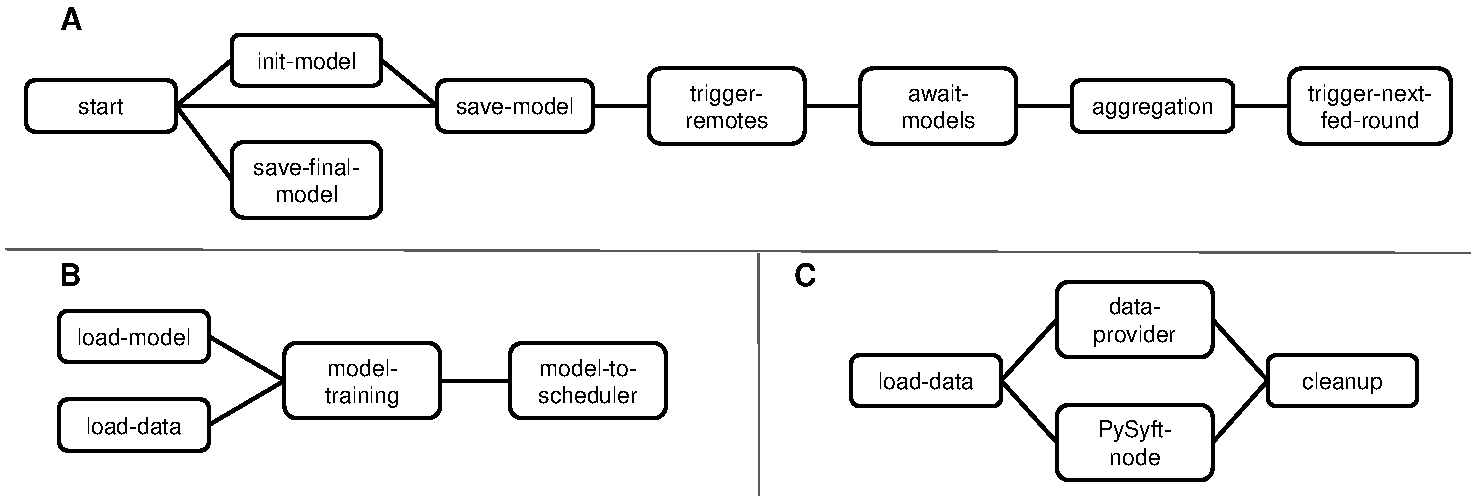
\includegraphics[width=1\textwidth]{1_Figures/dags.pdf}}
    \caption[DAGs for JIP Federated and the JIP's PySyft integration]{DAGs for JIP Federated (A \& B) and the JIP's PySyft integration (C). (A) DAG on central instance, which schedules the federated experiment and its individual process steps. (B) DAG on a participating institutions, which loads the local data and the consensus model from the central instance to execute the model training. When training is completed, the updated model is saved back to the central instance.  (C) DAG on a participating instance loading and providing its locally available data to the PySyft-Node, which then executes the computations during training. Note that the central instance of the PySyft integration hosts its PySyft-Notebook without being integrated into a DAG.}
\label{fig:Dags}
\end{figure}

% ### scheduler dag ####
The workflow on the central instance controls the processes of the experiment and can be described as follows (see \Cref{fig:Dags} A).
First, depending on the current round, either a new model is initialized  or the model of the previous round is directly stored into the object store.
In case it was the last round, the experiment is completed. Otherwise, it continues with the next operator.
% API Calls & Waiting
After saving the model, API calls are triggered on the participants' sites in order to start the corresponding training DAGs there. The relevant training information is also passed on to the participants. Subsequently, the workflow waits for the participants to send the models back to the central instance's object store. A regular check is made via the object store's its API to see whether all awaited models have already arrived.
% aggregation
When this is the case, the following operator performs the model aggregation and constructs the consensus model.
% completion
Before completing the current workflow, the DAG triggers itself for another run. Required data and information, such as the current federated round, are passed on to the next DAG. Thus, one federated round is represented by one run of the DAG on the central instance.

% training dag
At each participating clinic, identical training DAGs are implemented (see \Cref{fig:JIP} B).
The DAG starts with loading the data into Airflow. In parallel, a second operator accesses the object store of the central instance and loads the model from the previous round directly from there.
The operator to train the model brings the loaded data and model together and executes the training. After the local training is completed, the last operator saves the model back into the object store on the central instance.

% Usability
Due to the modularity of the DAGs, the individual operators can be reused for other experiments. In most cases, a developer only needs to customize the experiment-specific operators for model aggregation and model training on the nodes to implement a new experiment.
%Apart from the operators for the experiments, all others are reusable in their current implemented form for further experiments. So a developer only needs to customize the operators for aggregation and training on the nodes to implement the new experiment.


\subsection{Development}
\label{subsec:Development} 

% Intro & General
In the following, the implementations of the JIP's PySyft integration and JIP Federated are described in detail.
The implementations are publicly available on GitHub embedded in the Kaapana project---the JIP's PySyft integration can be found on the branch \textit{feature/openmined}\footnote{\url{https://github.com/kaapana/kaapana/tree/feature/openmined}\\ commit hash: aab58dac046f22d1b67ee2b49d9f4c72f7b0b69d}, JIP Federated on the branch \textit{feature/federated-training}\footnote{\url{https://github.com/kaapana/kaapana/tree/feature/federated-training}\\ commit hash: 1da26c0dfbe53d3a092762bd8e8a9e2e564148ef}.

% Minio Operator 
A central operator is the \textit{LocalMinioOperator}\footnote{\url{https://github.com/kaapana/kaapana/blob/develop/workflows/airflow-components/plugins/kaapana/operators/LocalMinioOperator.py}}. It serves as an interface between the Airflow environment and the object-store MinIO. The operator can be used for applying the operations \textit{get}, \textit{remove}, and \textit{put} on the buckets and available files. Across both implementations and all experiments, it is used, for instance, to load data into the Airflow environment or to load and store models.
% (\verb|get|, \verb|remove|, \verb|put|)

% ### PySyft ###
\subsubsection{PySyft Integration into the JIP}

% central instance
The three containerized PySyft components (PySyft-Notebook, PySyft-Grid, PySyft-Notebook) are embedded into the JIP via Helm charts\footnote{\url{https://github.com/kaapana/kaapana/tree/feature/openmined/services/applications/openmined}}. This allows to install them via the JIP's GUI as a JIP extension. \textit{PySyft-Grid} and \textit{PySyft-Notebook} are installed as such extensions on the central instance.
% participants
On the participants, the \textit{PySyft-Node} is integrated into a DAG\footnote{\url{https://github.com/kaapana/kaapana/blob/feature/openmined/workflows/airflow-components/dags/dag_openmined_provide_data.py}} which is depicted in \Cref{fig:DetailedDAG_PySyft}. In addition to an operator to load the data into the Airflow environment, the following three operators are implemented for this DAG.

% run-node-operator
The \textit{RunNodeOperator} is implemented as \textit{Application-Operator}. These operators can launch applications via the Helm API, similar to manually installing an extension. By running this operator, the \textit{PySyft-Node} is started as a temporary application in the JIP. This is done in parallel with the operator described next.

% provide-data-operator
The \textit{ProvideDataOperator} starts a Docker container\footnote{\url{https://github.com/kaapana/kaapana/tree/feature/openmined/workflows/processing-container/openmined/provide-data}}, which mounts the directory containing the previously loaded data. When the container is launched, it executes its process script. Meaning that data is loaded, transformed, tagged, and then sent to the \textit{PySyft-Node}. A parameter can be set for how long the data should be provided into the node.

% shutdown
When the previous operator is completed, the subsequent \textit{ShutdownNodeOperator} is launched to call the Helm API to uninstall \textit{PySyft-Node} chart.
From this point on, the node is unsubscribed from the \textit{PySyft-Grid} and its data is not hosted any further. As a last step, the used Airflow directories are emptied.

\begin{figure}[htbp!]
    \centerline{\includegraphics[width=1\textwidth]{1_Figures/DAG_PySyft.pdf}}
    \caption[Detailed illustration of DAG for the JIP's PySyft integration]{Detailed DAG of the JIP's PySyft integration for providing locally available data of participating institutes}
\label{fig:DetailedDAG_PySyft}
\end{figure}

% Operators 
The operators used for the JIP's PySyft integration are can be found in the repository\footnote{\url{https://github.com/kaapana/kaapana/tree/feature/openmined/workflows/airflow-components/dags/openmined}}.
Exemplary experiment-notebooks are made available together with the Docker image of the \textit{PySyft-Notebook} component\footnote{\url{https://github.com/kaapana/kaapana/tree/feature/openmined/workflows/processing-container/openmined/provide-data}}.



% ### JIP Federated ###
\subsubsection{JIP Federated}
\label{subsubsec:JIPFederated}

As described in \Cref{subsec:MethodsJIPFederated} (see \pageref{subsec:MethodsJIPFederated}, each experiment using JIP Federated is based on two DAGs\footnote{\url{https://github.com/kaapana/kaapana/tree/feature/federated-training/workflows/airflow-components/dags}}---one implemented on the central instance and the second on the participating institutions. \Cref{fig:DetailedDAG_KaapanaFed} provides a detailed illustration of the two DAGs.
In the following, the implemented operators are described in detail---the source-code is publicly available\footnote{\url{https://github.com/kaapana/kaapana/tree/feature/federated-training/workflows/airflow-components/dags/federated_training}}.
The same applies to the corresponding processing containers\footnote{\url{https://github.com/kaapana/kaapana/tree/feature/federated-training/workflows/processing-container/federated-training}}.
Note that depending on whether \textit{aggregation} or \textit{sequential training} was chosen as computing plan, the behavior of the operators slightly differ.

\textit{EntrypointOperator} is the first operator being executed when the DAG starts. Given the parameter provided by the API call of the data scientist or the previous DAG-run, it determines the next step. 
For the first federated round, the first model is initialized. In case the training is completed, the next step is to save the final model and finalize the workflow.
Otherwise, the training continues and the model from the previous round is saved to MinIO.
The routing is realized by the \textit{KaapanaBranchPythonBaseOperator} which branches the workflow depending on the information given the information received from the \textit{EntrypointOperator}.

\textit{ExperimentOperator} is used at two points in the DAG. First, it initializes the model in the first round. Further, it is used for aggregation of models received from the participants. When a \textit{sequential} computing plan is applied, the model is simply loaded and directly saved again to the target directory.
To decide between the tasks to be executed, corresponding parameters are passed when starting the operator.
While all other operators are generic, this operator is experiment-specific. The specific operators for each of the conducted experiments are also available in the repository and can be identified by their name (i.e. \verb|ExperimentsBraTSOperator.py|).

\textit{TriggerRemoteWorkersOperator} triggers the DAGs on the participating institutes. For each participant, an API call is executed which contains the required information and parameters, such as current federated round, number of epochs to train locally, and learning rate to use. In addition, information about the central instance is provided so that an allocation can be done. Note that no model is sent by the central instance.
In parallel, a \textit{LocalMinioOperator} empties the model cache in MinIO, because the new models of the participants are expected there.

\textit{AwaitingModelsOperator} is used to keep the workflow waiting for the models to be sent back. It uses the API of MinIO to check every three seconds whether the models of the participants have already arrived in the model cache (which has been emptied before to guarantee that no models from earlier rounds are used). As soon as all newly updated models are available, the loop ends and the operator completed its task.

\textit{TriggerMyselfOperator} is the final operator of the DAG.
It serves for launching the next Dag-Run. For this, it transfers the required data, such as the current model

\begin{sidewaysfigure}[htbp]
    \centerline{\includegraphics[width=1\textwidth]{1_Figures/DAG_KaapanaFed.pdf}}
    \caption[Detailed illustration of DAGs for JIP Federated]{DAGs for JIP federated. (A) DAG on the central instance, scheduling the overall workflow. (B) Training DAG implemented on the participating instances.}
\label{fig:DetailedDAG_KaapanaFed}
\end{sidewaysfigure}

checkpoint, into a newly created folder for the following DAG run. The operator also applies a new API call based on the previous call and therefore triggers the next round. In case of a \textit{sequential} computing plan, this operator determines which participant is next to receive the model for training. In addition, the operator manages the incrementing of the performed federated rounds depending on the applied computing plan.

For the model training on the participating institutes, the following operators are used for the corresponding DAG.
When the DAG is externally triggered by the central instance' \textit{TriggerRemoteWorkersOperator}, two \textit{LocalMinioOperator} are started to load the locally available data and the model into the Airflow environment. Note that the model is loaded directly from the object store of the central instance---this actually implies that the model is not sent to but pulled by the participants.
% Training Operator

\textit{TrainingOperator} launches a Docker container which accesses the loaded data and model.  The container executes a processing script which is similar to a regular PyTorch experiment. Data transformations are applied, and the model is trained for the given number of epochs.
As before, these experiment-specific operators can be identified by their name (i.e. \verb|TrainingBraTSOperator.py|).

% save back to central instance
When the training is completed, another \textit{LocalMinioOperator} is used to store the updated model again directly into the object store of the central instance.
This completes the DAG on the participant. Depending on the configuration, checkpoints of the model can also be saved locally on the participant.


\subsection{Experiments, Algorithms \& Datasets}
\label{subsec:MethodsExperiments}

Two classification experiments were carried out to compare the JIP's PySyft integration and JIP Federated. These experiments aim to compare the runtime and thus the efficiency of the two solutions while achieving similar learning behavior and performance. Additionally, a segmentation experiment on complex multi-modal medical images was conducted to demonstrate the capabilities JIP Federated. 
We demonstrate that it is feasible to perform FL with the JIP on a standard benchmark dataset of medical brain tumor scans.
% General setting with three participants (in all experiments)
For all experiments, we assume that three participating institutes provide their local data. Furthermore, in every federated round one epoch is trained on the available data.

% ### Runtime Experiments ###
The runtime experiments were conducted on two different publicly available datasets: the widely known Modified National Institute of Standards and Technology\footnote{\url{http://yann.lecun.com/exdb/mnist/}} (MNIST) \citep{LeCunYannandCortesCorinnaandBurges2010} dataset, consisting of 70,000 digit handwriting images (60,000 for training and 10,000 for testing), and the paediatric pneumonia dataset\footnote{\url{https://data.mendeley.com/datasets/rscbjbr9sj/3}} originally proposed by \cite{Kermany2018IdentifyingLearning}. It contains paediatric chest radiographs split into 5,232 samples for training and 624 for testing. The data is classified as either normal (with no signs of infection, 1,349 samples) or infected (bacterial or viral pneumonia, 3.883 samples). The test data contains 234 normal samples and 390 samples classified as infected. In order to use the datasets in a federated setting, non-overlapping subsets were formed. Each class in the training data was randomly divided into three parts and distributed among the participants. The test data was held out for final global testing after training. This process was applied on both datasets.
% dataset class distribution 
% total:    5,232 (3,883 pneumonia, 1,349 normal)
% training: ...
% testing:  624 (390 pneumonia, 234 normal)

% Applied transformations
Before the samples of the two datasets were used for training, image transformations were applied. While the MNIST images were only normalized, the following transformations were performed on the pneumonia images.
Image resizing to $256 \times 256$ pixels,
random horizontal flipping,
random vertical flipping,
and image normalization.

For the MNIST experiments, the algorithm and training parameters were adopted from the basic MNIST example of PyTorch\footnote{\url{https://github.com/pytorch/examples/blob/master/mnist/main.py};\\commit hash: 0f0c9131ca5c79d1332dce1f4c06fe942fbdc665}. Training was performed for 14 federated rounds using a batch size of 64 and a learning rate of $10^{-2}$. For the experiment on pneumonia radiographs, the ResNet18 (see \cite{He2016DeepRecognition}) architecture pre-trained on ImageNet was used, following \cite{Kaissis2021End-to-endImaging}. The model was trained for 40 federated rounds with a learning rate of $10^{-4}$ and a batch size of 8 (also used by the baseline for the processing time experiments in \cite{Kaissis2021End-to-endImaging}). Due to PySyft's limitation of not supporting momentum terms in the integrated release version, Stochastic Gradient Descent (SGD) was used as optimizer.
% Kaissis Baseline: "All times shown in white are relative to the baseline for a batch size of 8" - Haben sie als Baseline genutzt um den Zeitaufwand zu vergleichen

% ACCURACY
To measure the performance of the trained models on the test data, the metric \textit{Accuracy} was used. Its value represents the proportion of the correctly classified samples over all samples. The metric is defined as:
\begin{equation}
Accuracy=\frac{TP + TN}{TP + TN + FP + FN} \label{eq:accuracy}
\end{equation}
where TP = True Positive, FP = False Positive, TN = True Negative, FN = False Negative.
% AU-ROC
In addition, the area-under-the-receiver-operator-characteristic (AUROC) is measured for the experiments on the slightly imbalanced pneunomia dataset.
The metric is a performance metric based on the receiver-operator-characteristic (ROC) curve, which represents possible combinations of true-positive-rate (TPR) and the false-postive-rate (FPR).
By mapping the FPR on the x-axis and the TPR on the y-axis, a curve is formed. The area underneath this curve is the AUROC and its value ranges between 0 and 1 (higher is better). 

% Furthermore, the integrated PySyft version does not support graphical processing unit (GPU), thus, the experiments were carried on central processing unit (CPU) resources only.
Furthermore, all JIP instances for the experiments were set up identically, and training was carried out on the central processing unit (CPU). Computing resources of 10,000 Mi\footnote{\unexpanded{$1\ Mi\ (mebibyte) = 1024 \times 1024\ bytes$}} were allocated to each node, respectively training container, by the underlying Kubernetes.


% ### BraTS ###

In the federated segmentation experiment with JIP Federated, a U-Net \citep{Ronneberger2015U-net:Segmentation} was trained to segment diagnosed gliomas in MRI scans of human brains. The U-Net architecture was set up with a channel sequence of ($16, 32, 64, 128, 256$) and convolution strides of size two. The number of residual units was set to two.
The results and training behavior is compared to an experiment where an identical U-Net architecture was trained on the centralized data using the same hyperparameter configuration.
In both cases, the models were trained for 500 epochs, respectively federated rounds. Each federated round consisted of one local epoch on each of the participants.
% GPU
The model training computations were performed on graphical processing units (GPUs).
% Dataset description
The brain dataset from the \textit{Medical Segmentation Decathlon} was used. The dataset consists of a subset of the Brain Tumor Segmentation (BraTS) \cite{Menze2015TheBRATS} Challenge 2016 and 2017 data \citep{Antonelli2021TheDecathlon}. Besides unlabeled test samples, it contains 484 multi-modal MRI scans and their corresponding labels. 96 of the labeled samples were separated to serve as test data for measuring the model performance. For the experiment, three participating sites were established on individual server instances. Accordingly, the data was randomly sampled and divided into three non-overlapping subsets. Each instance was provided with 129 samples for training and 32 for testing. For centralized training, the identical data was merged into central datasets and then used for training and testing.
% bezeichnung der Daten <-- clear naming! 
In the remainder of this work, this data will be referred to as BraTS dataset.

% optimizer & reference to appendix for details
To train the model with this data, we used the Adam optimizer \citep{Kingma2014Adam:Optimization} with a 
learning rate of $10^{-4}$
and weight decay of $10^{-5}$.
% Applied transformations
For the model training, the brain scans undergo the following transformations.
Random vertical flipping,
random spacial cropping ($\textrm{with roi\_size} =  128 \times 128 \times 64$),
intensity normalization,
random intensity shifting,
and random intensity scaling.
% ref to MONAI Tutorial
The parameters of the optimizer, the applied transformations, and the U-Net architecture were adopted from the 3D brain segmentation tutorial\footnote{\url{https://github.com/Project-MONAI/tutorials/blob/master/3d\_segmentation/brats\_segmentation\_3d.ipynb}; commit hash: d340613cea8b0f10b780694c636c1d7ff8f7658d}
%\footnote{https://github.com/Project-MONAI/tutorials}
of the Medical Open Network for AI (MONAI) Project\footnote{\url{https://monai.io/}}. After each federated round, the models are aggregated by applying \textit{Federated Averaging}.

% Optimizer state handling (keep local, agg, reset) --> Das hier ist neu!
When models are aggregated into a consensus model, the question of how to handle the used optimizer arises. For this \textit{optimizer state treatment}, three methods are apparent. As with the model, a consensus optimizer state could be derived from averaging the states of the participants. Alternatively, the optimizer state could be kept on the local instance only or reset for each new federated round. Based on the results shown in the work of \cite{Li2019Privacy-preservingSegmentation}, we decided to also reset the optimizer state before continuing a new federated round.
% sheller gibt nur die Werte für RESET und HOLD an - die sind sehr ähnlich, wie deutlich AGG besser ist wird nicht gesagt. Ich lasse Sheller weg, weil Li klar die Aussage trifft (und auch eben BraTS macht)
% \cite{Li2019Privacy-preservingSegmentation}: "For the treatment of momentum variables, restarting them at each federated round outperforms all the other variants" 

% Dice Score explaining!
As in all BraTS challenges, the \textit{Dice Coefficient} (DC) was used for the quantitative performance evaluation of the model.
This metric measures the overlap of two binary segmentation masks and ranges from 0 to 1 (higher is better). DC is defined as:
\begin{equation}
DC=\frac{2 |P \cap T|}{|P| + |T|} \label{eq:dice}
\end{equation}
where P is the prediction and T the ground truth mask. The DC is measured for all three (overlapping) tumor regions\footnote{In the medical segmentation decathlon, the label convention slightly differs from BraTS.}:
\begin{itemize}
    \item Enhancing tumor (ET): label 2
    \item Tumor core (TC): labels 2 and 3
    \item Whole tumor (WT): labels 1, 2 and 3
\end{itemize}

\begin{comment}
\begin{enumerate}
    \item Enhancing tumor (ET): label 2
    \item Tumor core (TC): labels 2 and 3
    \item Whole tumor (WT): labels 1, 2 and 3
\end{enumerate}
\end{comment}

% Table summerazis the chosesn parameter configurartions for all conducted experiments.
\Cref{tab:TrainingParameters} summarizes the chosen parameter configurations for all conducted experiments.
Note that apart from the listed parameters, the Adam optimizer was used with its PyTorch default values for the segmentation experiment.

\begin{table}[htbp]
\begin{adjustbox}{width=1.0\textwidth}
  \centering
  \begin{tabular}{ccccccc}
  Experiment & Federated Rounds & Epochs per Round & Optimizer & Batch Size & Learning Rate & Weight Decay \\
  \hline \\[-2.5ex] %[-1.5ex]
  MNIST     & 14    & 1 & SGD   & 64 & $10^{-2}$ & - \\
  Pneunomia & 40    & 1 & SGD   & 8  & $10^{-4}$ & - \\
  BraTS     & 500   & 1 & Adam  & 2  & $10^{-4}$ & $10^{-5}$ \\
 \end{tabular}
 \end{adjustbox}
 \caption[Training parameters for conducted FL experiments]{Training parameters for conducted FL experiments on MNIST, pneumonia and BraTS data}
 \label{tab:TrainingParameters}
\end{table}

 
 \section{Results}
\label{sec:Results}

\subsection{Requirements \& Comparison of FL Solutions}
\label{subsec:ResultsRequirements}

% Reference to the table
\Cref{tab:ToolComparison} summarizes the results of our requirement analysis and the comparison of the FL solutions considered in this work. The identified requirements are described in more detail in the following. Please note that entries marked with a hyphen could not be determined with full confidence by the author team\footnote{Not all the available resources are detailed enough to allow a reliable classification.}.
The two entries marked by additional brackets are explained in \Cref{subsec:DiscussionRequirements} (see page \pageref{subsec:DiscussionRequirements}).


\begin{sidewaystable}[htbp]
\centering
\begin{adjustbox}{width=0.8\textheight}
%\begin{adjustbox}{width=0.8\textwidth}
  \begin{tabular}{llccccccc}
    \multicolumn{2}{c}{Requirement} & TFF & FedML & FATE & PaddleFL & PySyft & \makecell{NVIDIA Clara \\ Federated} & \makecell{JIP \\ Federated} \\
    \hline \\[-2.5ex] %[-1.5ex]
    
    \multicolumn{2}{l}{Open-source}                                             & \cmark & \cmark & \cmark & \cmark & \cmark & \xmark & \cmark \\
    \multicolumn{2}{l}{Offline installation}                                    & \xmark & \xmark & \xmark & \xmark & \xmark & \cmark & \cmark \\
    
    %multi-rows
    \arrayrulecolor{lightgray} \hline \\ [-1.5ex]
    \multirow{2}{*}{Type of solution}   & Platform Solution                     &   &   &   &   &   & \cmark & \cmark \\
                                        & Programming Framework                 & \cmark & \cmark & \cmark & \cmark & \cmark &   &   \\
    \hline \\[-1.5ex]
    \multirow{2}{*}{GPU support}        & Single GPU                            & \cmark & \cmark & -      & \cmark & \xmark & \cmark & \cmark \\
                                        & Multiple GPUs                         & \cmark & \cmark & -      & \cmark & \xmark & \cmark & \cmark \\
    \hline \\[-1.5ex]
    \multirow{3}{*}{Data handling}      & Non-DICOM                             & \cmark & \cmark & \cmark & \cmark &  \cmark  & \cmark & \cmark \\
                                        & DICOM                                 & \xmark & \xmark & \xmark & \xmark & (\cmark) & \cmark & \cmark \\
                                        & PACS Connectivity                     & \xmark & \xmark & \xmark & \xmark &  \xmark  & \cmark & \cmark \\
    \hline \\[-1.5ex]
    \multirow{3}{*}{Privacy mechanisms} & Differential Privacy                  &(\cmark)& \xmark & \xmark & \cmark & \cmark & \cmark & \xmark \\
                                        & Homomorphic Encryption                & \xmark & \xmark & \cmark & \xmark & \cmark & \cmark & \xmark \\
                                        & Secure Multi-Party Computation        & \xmark & \cmark & \cmark & \cmark & \cmark & \xmark & \xmark \\
    \hline \\[-1.5ex]
    \multirow{3}{*}{DL frameworks}      & PyTorch                               & \xmark & \cmark & \cmark & \xmark & \cmark & \cmark & \cmark \\
                                        & TensorFlow                            & \cmark & \xmark & \cmark & \xmark & \cmark & \cmark & \cmark \\
                                        & PaddlePaddle                          & \xmark & \xmark & \xmark & \cmark & \xmark & -      & \cmark \\
    \hline \\[-1.5ex]
    \multirow{2}{*}{Compute plans}    & Aggregation                           & \cmark & \cmark & \cmark & \cmark & \cmark & \cmark & \cmark \\
                                        & Sequential                            & -      & -      & \cmark & \xmark & \cmark & \cmark & \cmark \\
    %                                   & Ensembling                            & -      & \xmark & -      & -      & \cmark & \cmark & \cmark \\
    \hline \\[-1.5ex]
    \multirow{2}{*}{Information}        & Documentation, Tutorials, \& Examples & \cmark & \cmark & \cmark & \cmark & \xmark & \cmark & \cmark \\
                                        & Community                             & \cmark & \cmark & \cmark & \xmark & \cmark & \cmark & \cmark \\
  \end{tabular}
  \end{adjustbox}
  \caption[Comparison of different FL solutions based on derived requirements for real-world FL with medical image data]{Comparison of different FL solutions based on derived requirements for real-world FL with medical image data. Note that entries marked with a hyphen could not be determined with full confidence. \cmark \space indicates that a requirement is fulfilled, \xmark \space indicates that it is not.}
  \label{tab:ToolComparison}
\end{sidewaystable}



% ### Federated Learning Requirements ###
From an FL perspective, the following requirements are derived.
% multiple compute plans possible
While applying \textit{model aggregation} is the most common compute plan, others such as \textit{sequential training} should be realizable in the solution \citep{Li2019Privacy-preservingSegmentation, Chang2018DistributedImaging}.
We therefore consider the ability to implement at least these two compute plans as a proxy for the flexibility of a solution, and include it as a requirement.

% privacy mechanisms
To maintain the data privacy and security of communication and thus the motivation behind FL, the solutions should provide \textit{privacy mechanisms} to address potential attacks and information leakage. While there might be further ones, we include the following mechanisms retrieved from \cite{Kaissis2020SecureImaging} in our comparison:
Differential Privacy \citep{Dwork2014ThePrivacy}, Homomorphic Encryption \citep{Acar2018AImplementation}, and Secure Multi-Party Computation \citep{Zhao2019SecureApplications}.
% "Secure Aggregation is a class of Secure Multi-Party Computation algorithms"

% ### Technical Requirements ###
Further, there are technical requirements that are practically important for FL solutions in the context of medical imaging.
% GPU support
Although it is possible to run computationally expensive experiments on the CPU, \textit{GPU support} is essential. This is particularly the case when dealing with image data, and even more when object segmentation is the given task \citep{Kaissis2021End-to-endImaging, Lee2021FederatedEnvironment}.
% DICOM format - medical imaging format & image data sets (multi-model dataset with arbitrary modality and dimension)
Another important requirement in a clinical setting is the  compatibility with medical \textit{image data formats}, such as \textit{Digital Imaging and Communication in Medicine} (DICOM) \citep{Kaissis2021End-to-endImaging}.
% PACS connectivity
In addition to the support of DICOM as data format, it is essential for the solutions' application in clinics that they  include an adapter to the \textit{Picture Archiving and Communication System} (PACS). PACS is the system for managing and archiving medical images and is connected to the clinic's imaging hardware.
% Open-source - proprietary - open-source / non proprietary solutions preferred
Because of the healthcare environment being highly sensitive, as well as individual for each site, solutions are required that are as flexible and adaptable as possible. In addition, the lock-in effect needs to be prevented. Therefore, it is relevant whether the solution is \textit{open-source} or proprietary from one provider.
% Offline installation
This is accompanied by an interest in the possibility of \textit{offline installation}, meaning that the solution is installable and runnable in an environment disconnected from the internet.
% Information
From a developer's perspective, it is also relevant to have \textit{information} about the solution's implementation and usage. Accordingly, we also include the availability of detailed documentation, tutorials, and an active user and developer community into our comparison.

% Solution: Platform vs. Coding Framework
Furthermore, we distinguish between two different \textit{types of solutions}. It can either be a programming framework, which comes with no or few surrounding features, or an extensive platform solution.






\subsection{Comparison of PySyft Integration \& JIP Federated}
\label{subsec:ResultsRuntime}

Based on the two classification experiments, we compare the JIP's PySyft integration and JIP Federated with regard to training duration. For a fair comparison, it must be ensured that both implementations result in similar training behavior and final performance.

\begin{figure}[htbp]
%\begin{figure}[h!]
    %\centerline{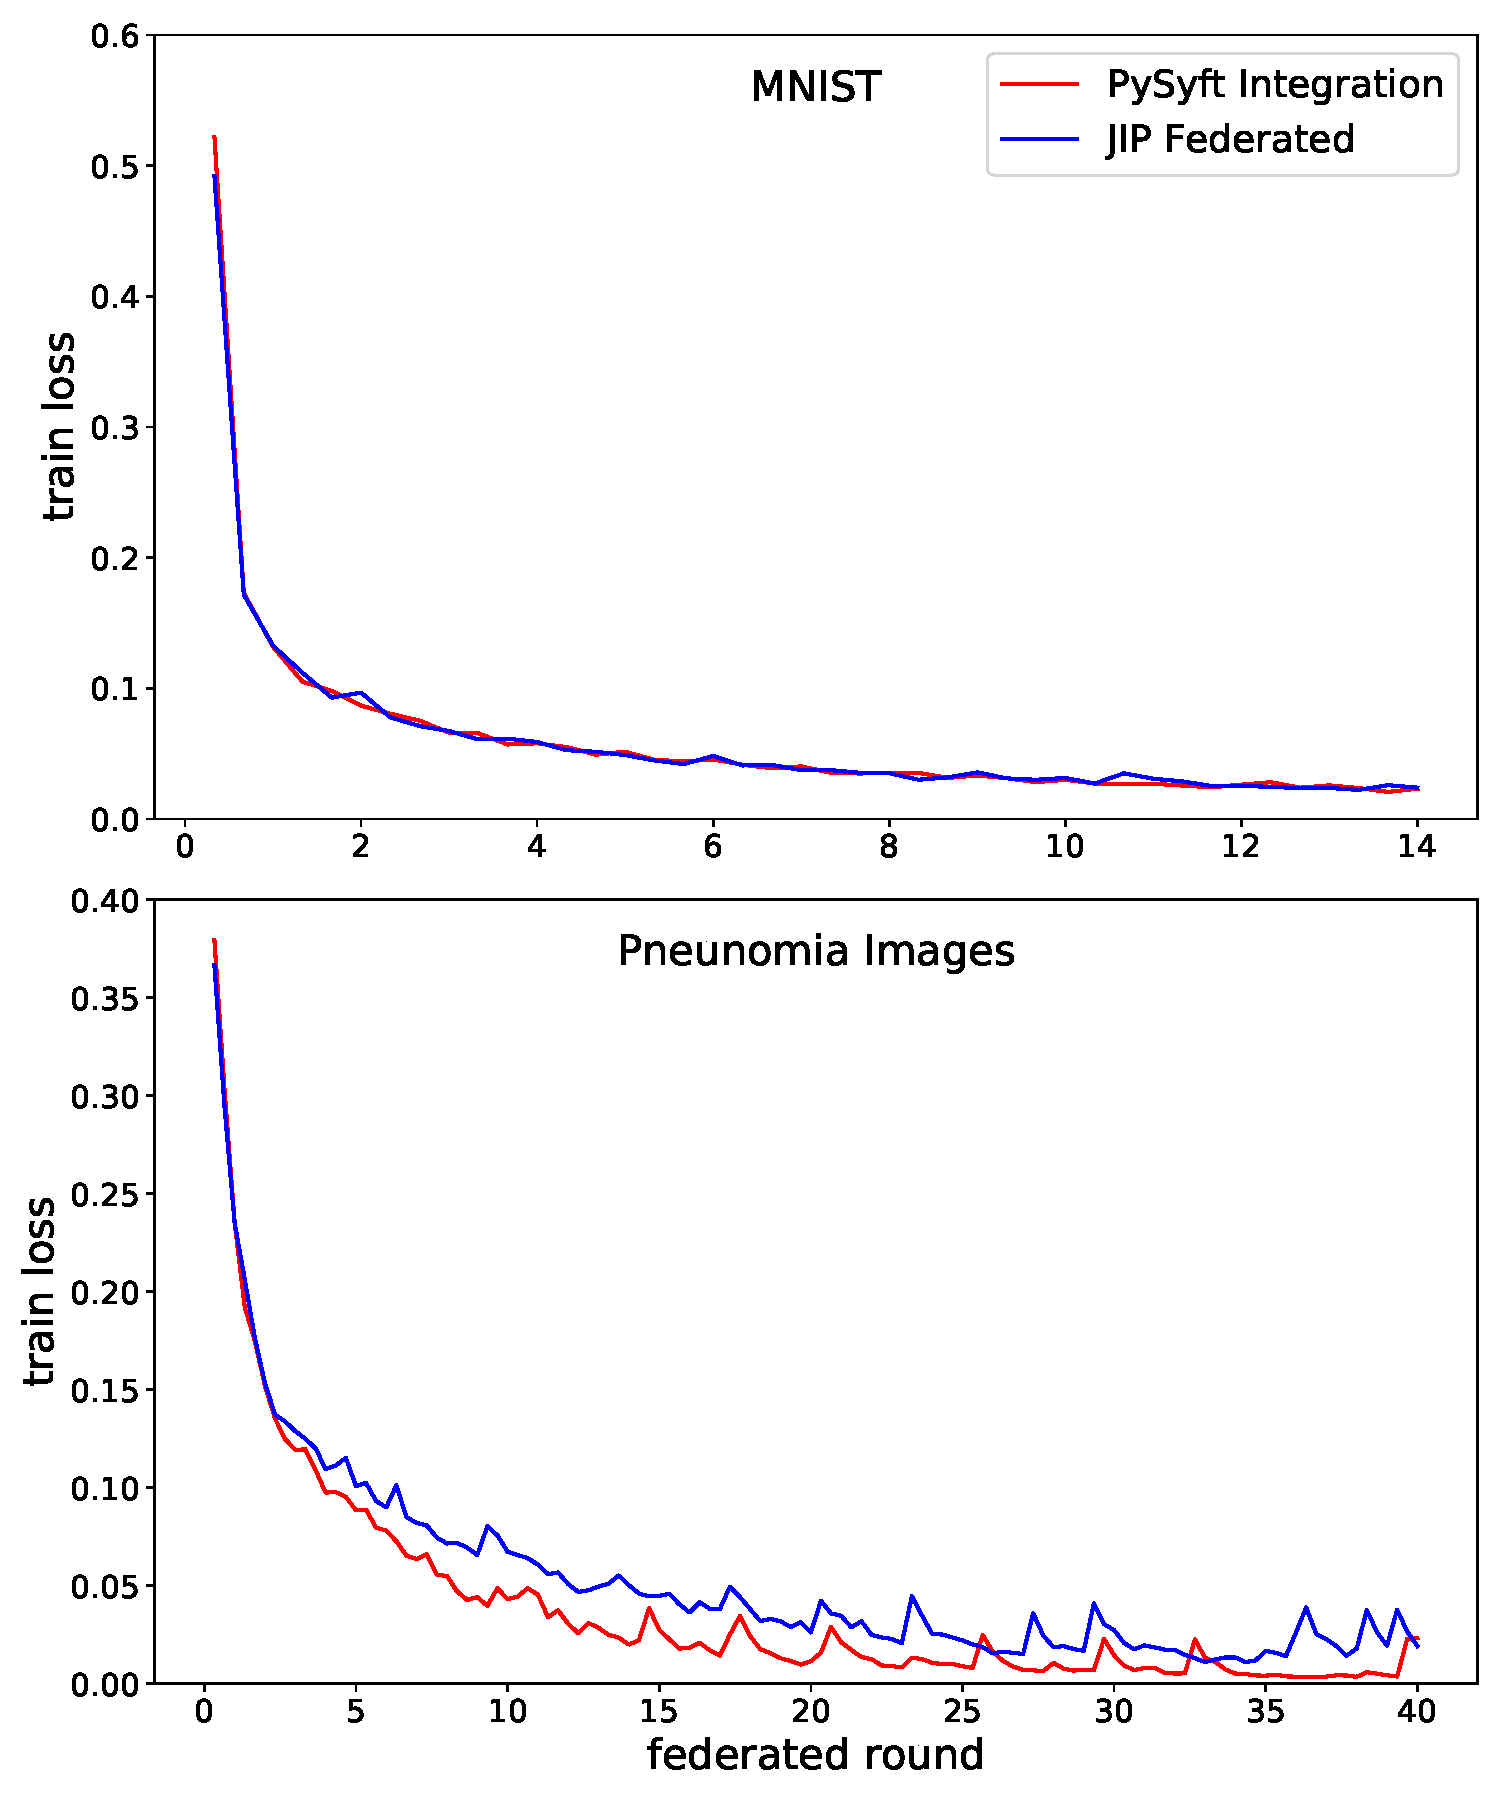
\includegraphics[width=1.0\textwidth]{1_Figures/RuntimeExperiments.pdf}}
    \centerline{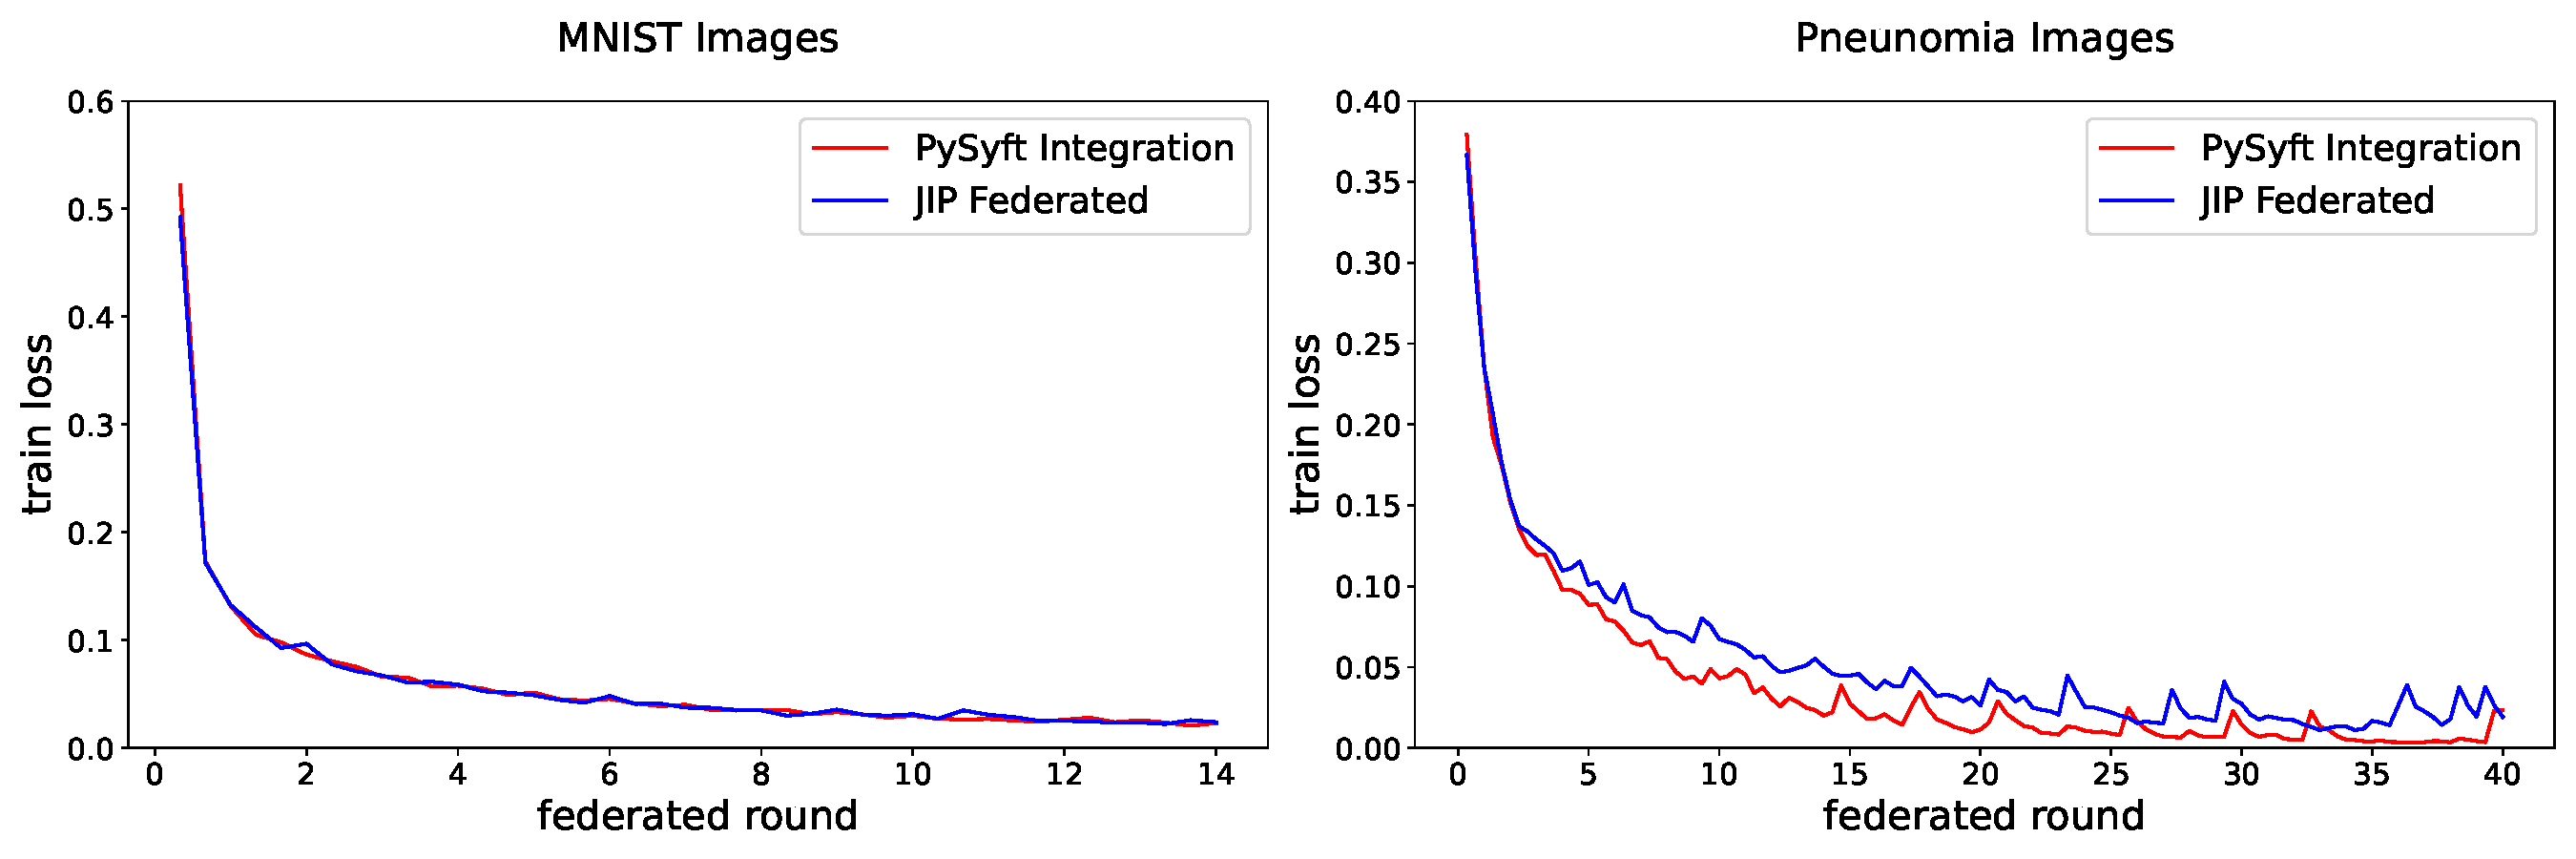
\includegraphics[width=1.0\textwidth]{1_Figures/RuntimeExperiments_horizontal.pdf}}
    \caption[Loss curves during model training on MNIST and pneunomia images]{Loss curves during model training on MNIST and pneumonia images using the JIP's PySyft integration (red) and JIP Federated (blue)}
\label{fig:RuntimeExp}
\end{figure}

\Cref{fig:RuntimeExp} illustrates the learning curves using the JIP's PySyft integration and JIP Federated when training on both datasets, MNIST and the pneumonia images. It shows the convergence when applying a \textit{sequential} compute plan. The depicted loss values represent the average values over the batch losses of one local epoch each.

\begin{table}[htbp]
  \centering
  \begin{tabular}{ccc}
  Experiment & Accuracy & AUROC \\
  \hline \\[-2.5ex] %[-1.5ex]
  PySyft on MNIST               & 99.02 \% & - \\
  JIP Federated on MNIST        & 99.20 \% & - \\
  PySyft on pneumonia           & 91.35 \% & 0.887 \\
  JIP Federated on pneumonia    & 92.79 \% & 0.906 \\
 \end{tabular}
 \caption[Performance scores on MNIST and pneunomia test data]{Performance scores on MNIST and pneumonia test data (one run)}
 \label{tab:Performance}
\end{table}
% PySyft MNIST:     99.02% 
% Kaapana MNIST:    99.20% 
% PySyft Chest:     91.346% (ROC-AUC: 0.887)
% Kaapana Chest:    92.788% (ROC-AUC: 0.906)

% Performance statistics
The performance of the final model checkpoints is compared using the accuracy on the held-out test data. 
For the experiments on the slightly unbalanced pneumonia dataset, the AUROC is considered additionally. The achieved scores are listed in \Cref{tab:Performance}.

%\begin{table}[h!]
\begin{table}[htbp]
  \centering
  \begin{tabular}{ccc}
  Implementation & MNIST & Pneumonia Images \\
  \hline \\[-2.5ex] %[-1.5ex]
  PySyft        & 01:46:32 & 20:51:21 \\
  JIP Federated & 01:38:50 & 08:55:03 \\
 \end{tabular}
 \caption[Runtime of conducted experiments on MNIST and pneunomia data]{Runtime of conducted experiments on MNIST and pneunomia data (hh:mm:ss; one run)}
 \label{tab:RuntimeExp}
\end{table}

% Run time
\Cref{tab:RuntimeExp} lists the runtime differences between starting the first federated round and saving the final model of the conducted experiment.




\subsection{JIP Federated Segmentation Experiment}
\label{subsec:ResultsSegmentation}

% Intro sentence
The segmentation experiment on the BraTS data serves to demonstrate that JIP Federated is capable of performing complex deep learning tasks.
% mean dice score and figure
\Cref{fig:BraTSplots} shows the training loss together with the dice scores on the three available segmentation masks (ET, TC, WT) described in \Cref{subsec:MethodsExperiments} (see page \pageref{subsec:MethodsExperiments}). In addition, the mean dice score built from the scores on the three segmentation masks is displayed.
The dice scores show the performance on the test data for each federated round, respectively epoch. Each data point represents the mean value over one iteration on the corresponding data.

% illustration
In order to imitate a realistic FL scenario, the test performance was computed locally on each participant using the test data available there. This results in three curves, depicted in gray, showing the local behavior. The local training loss and testing performance scores of the participating clinics were aggregated to averaged values depicted in red.
As upper baseline, the curves of the model training on the centralized data are displayed in blue.

%\begin{figure}[htbp]
\begin{figure}[t!]
    %\centerline{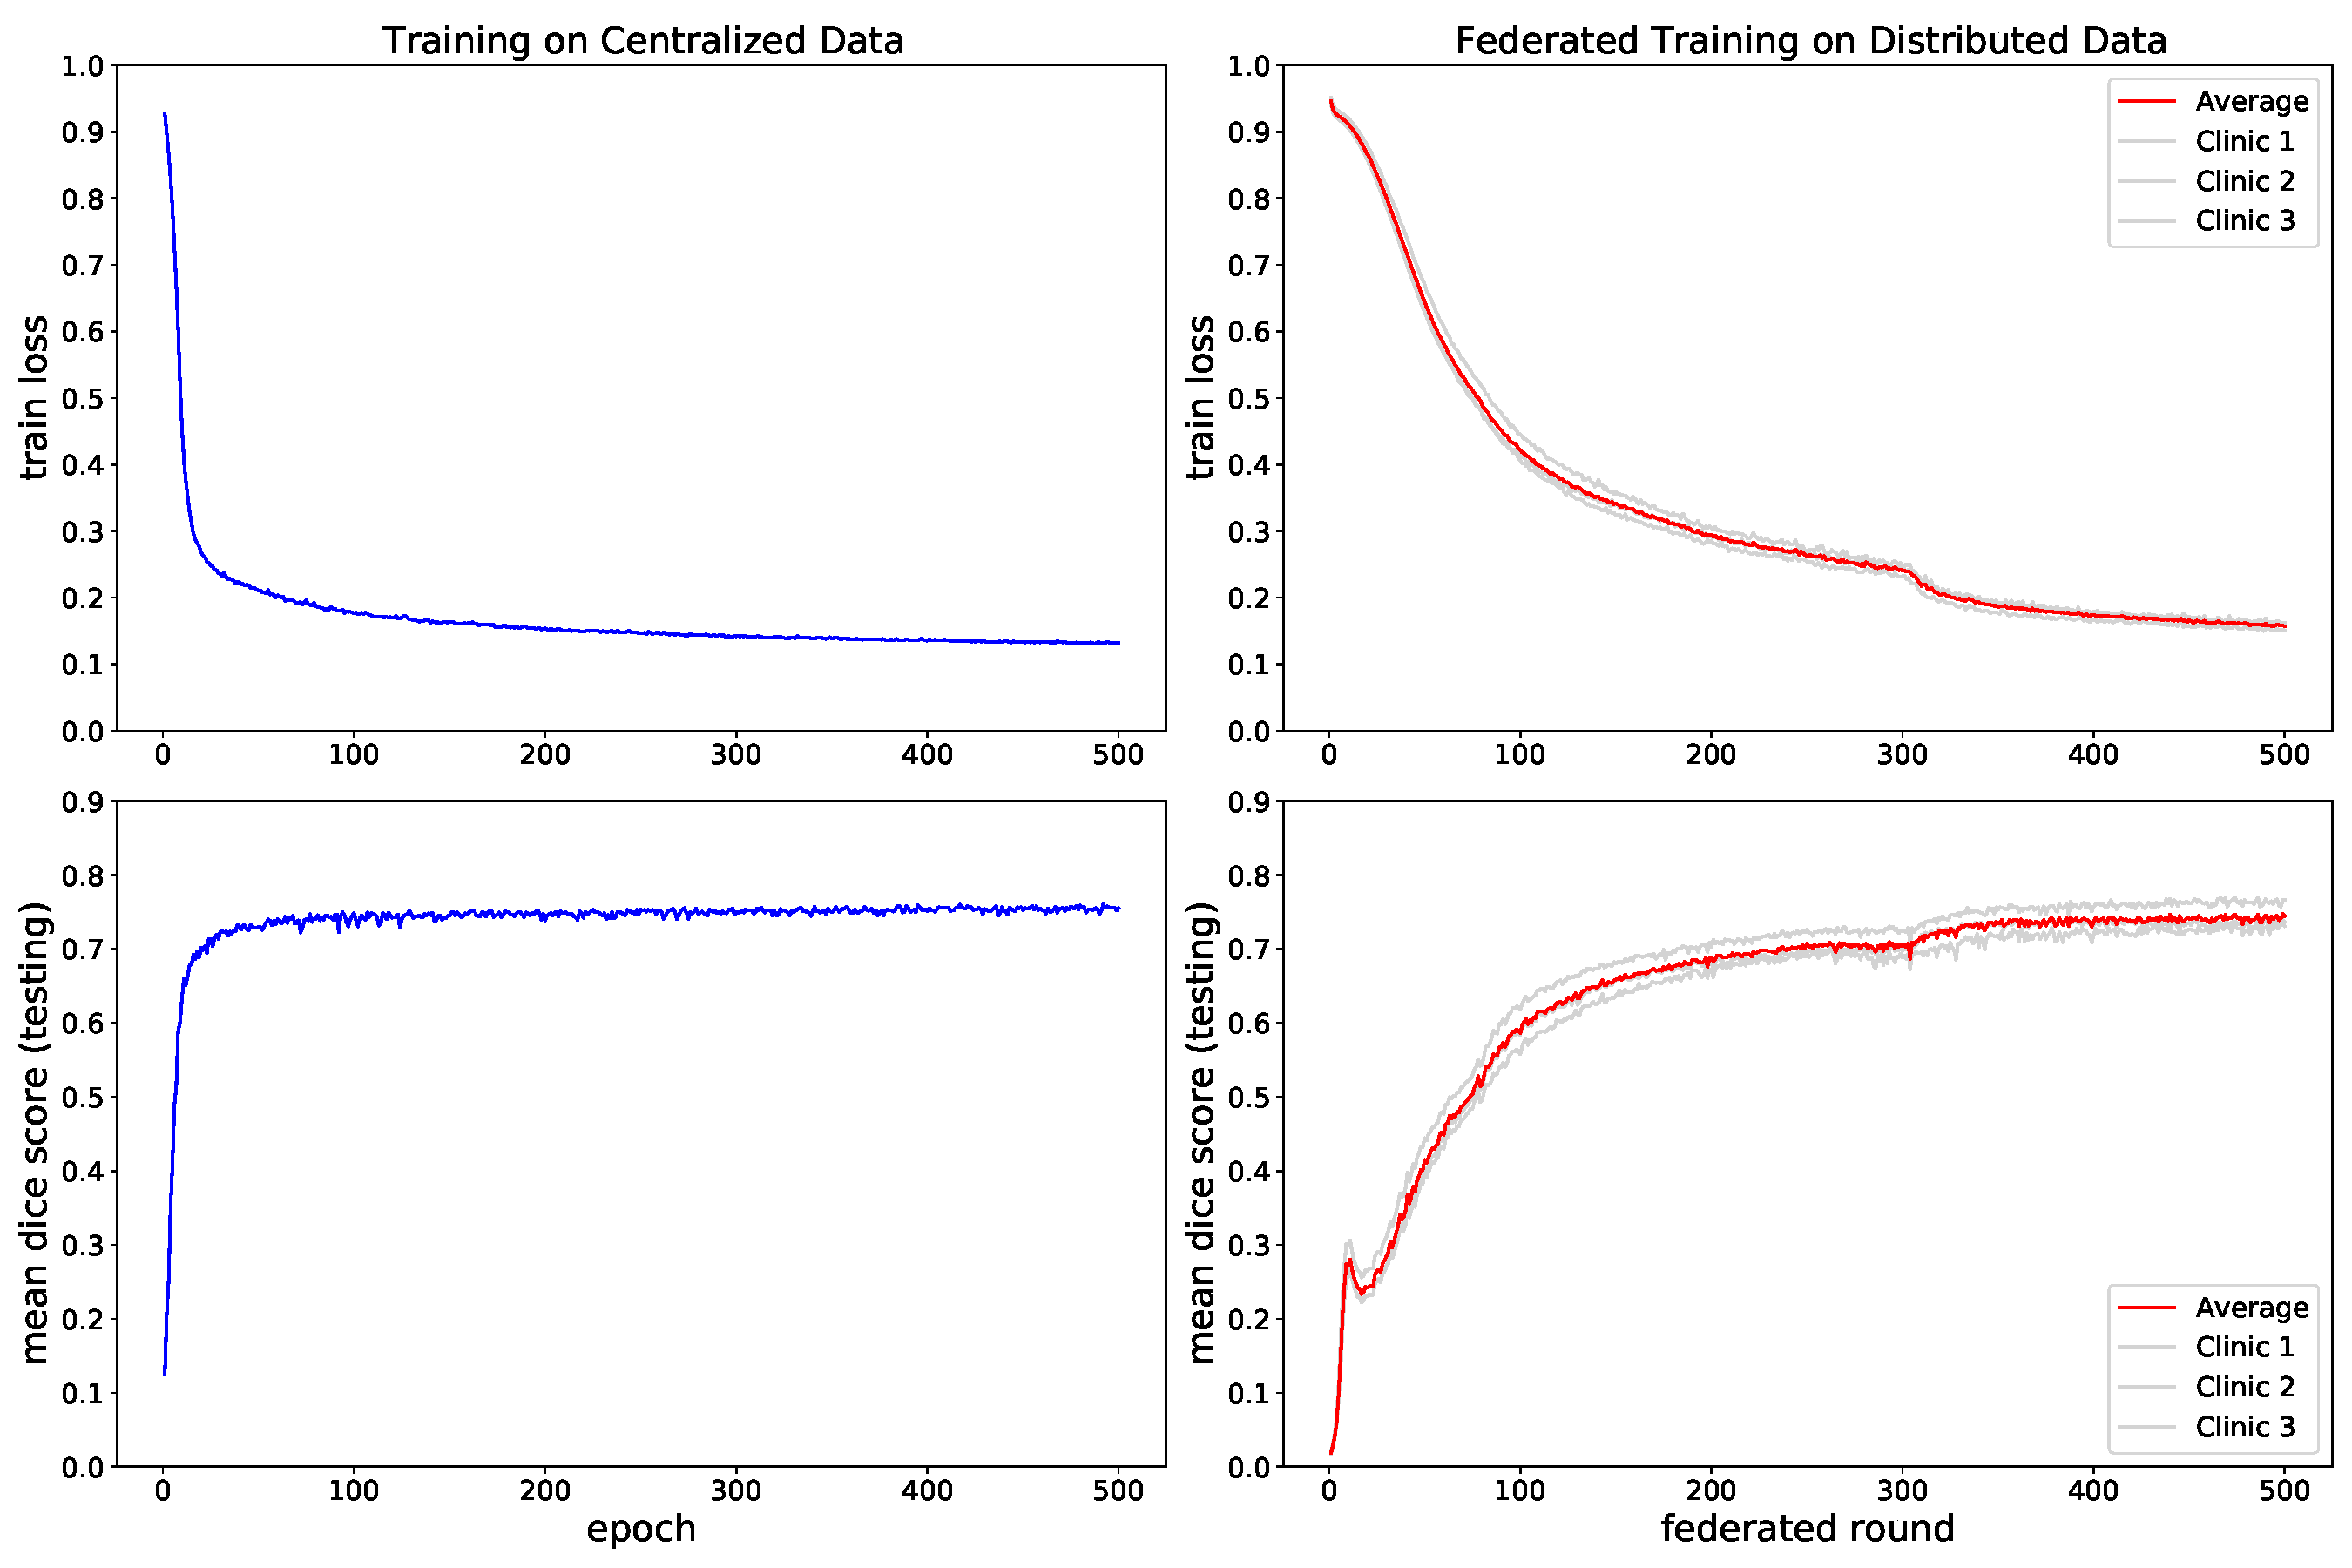
\includegraphics[width=1.0\textwidth]{1_Figures/BraTSexperiments.pdf}}
    \centerline{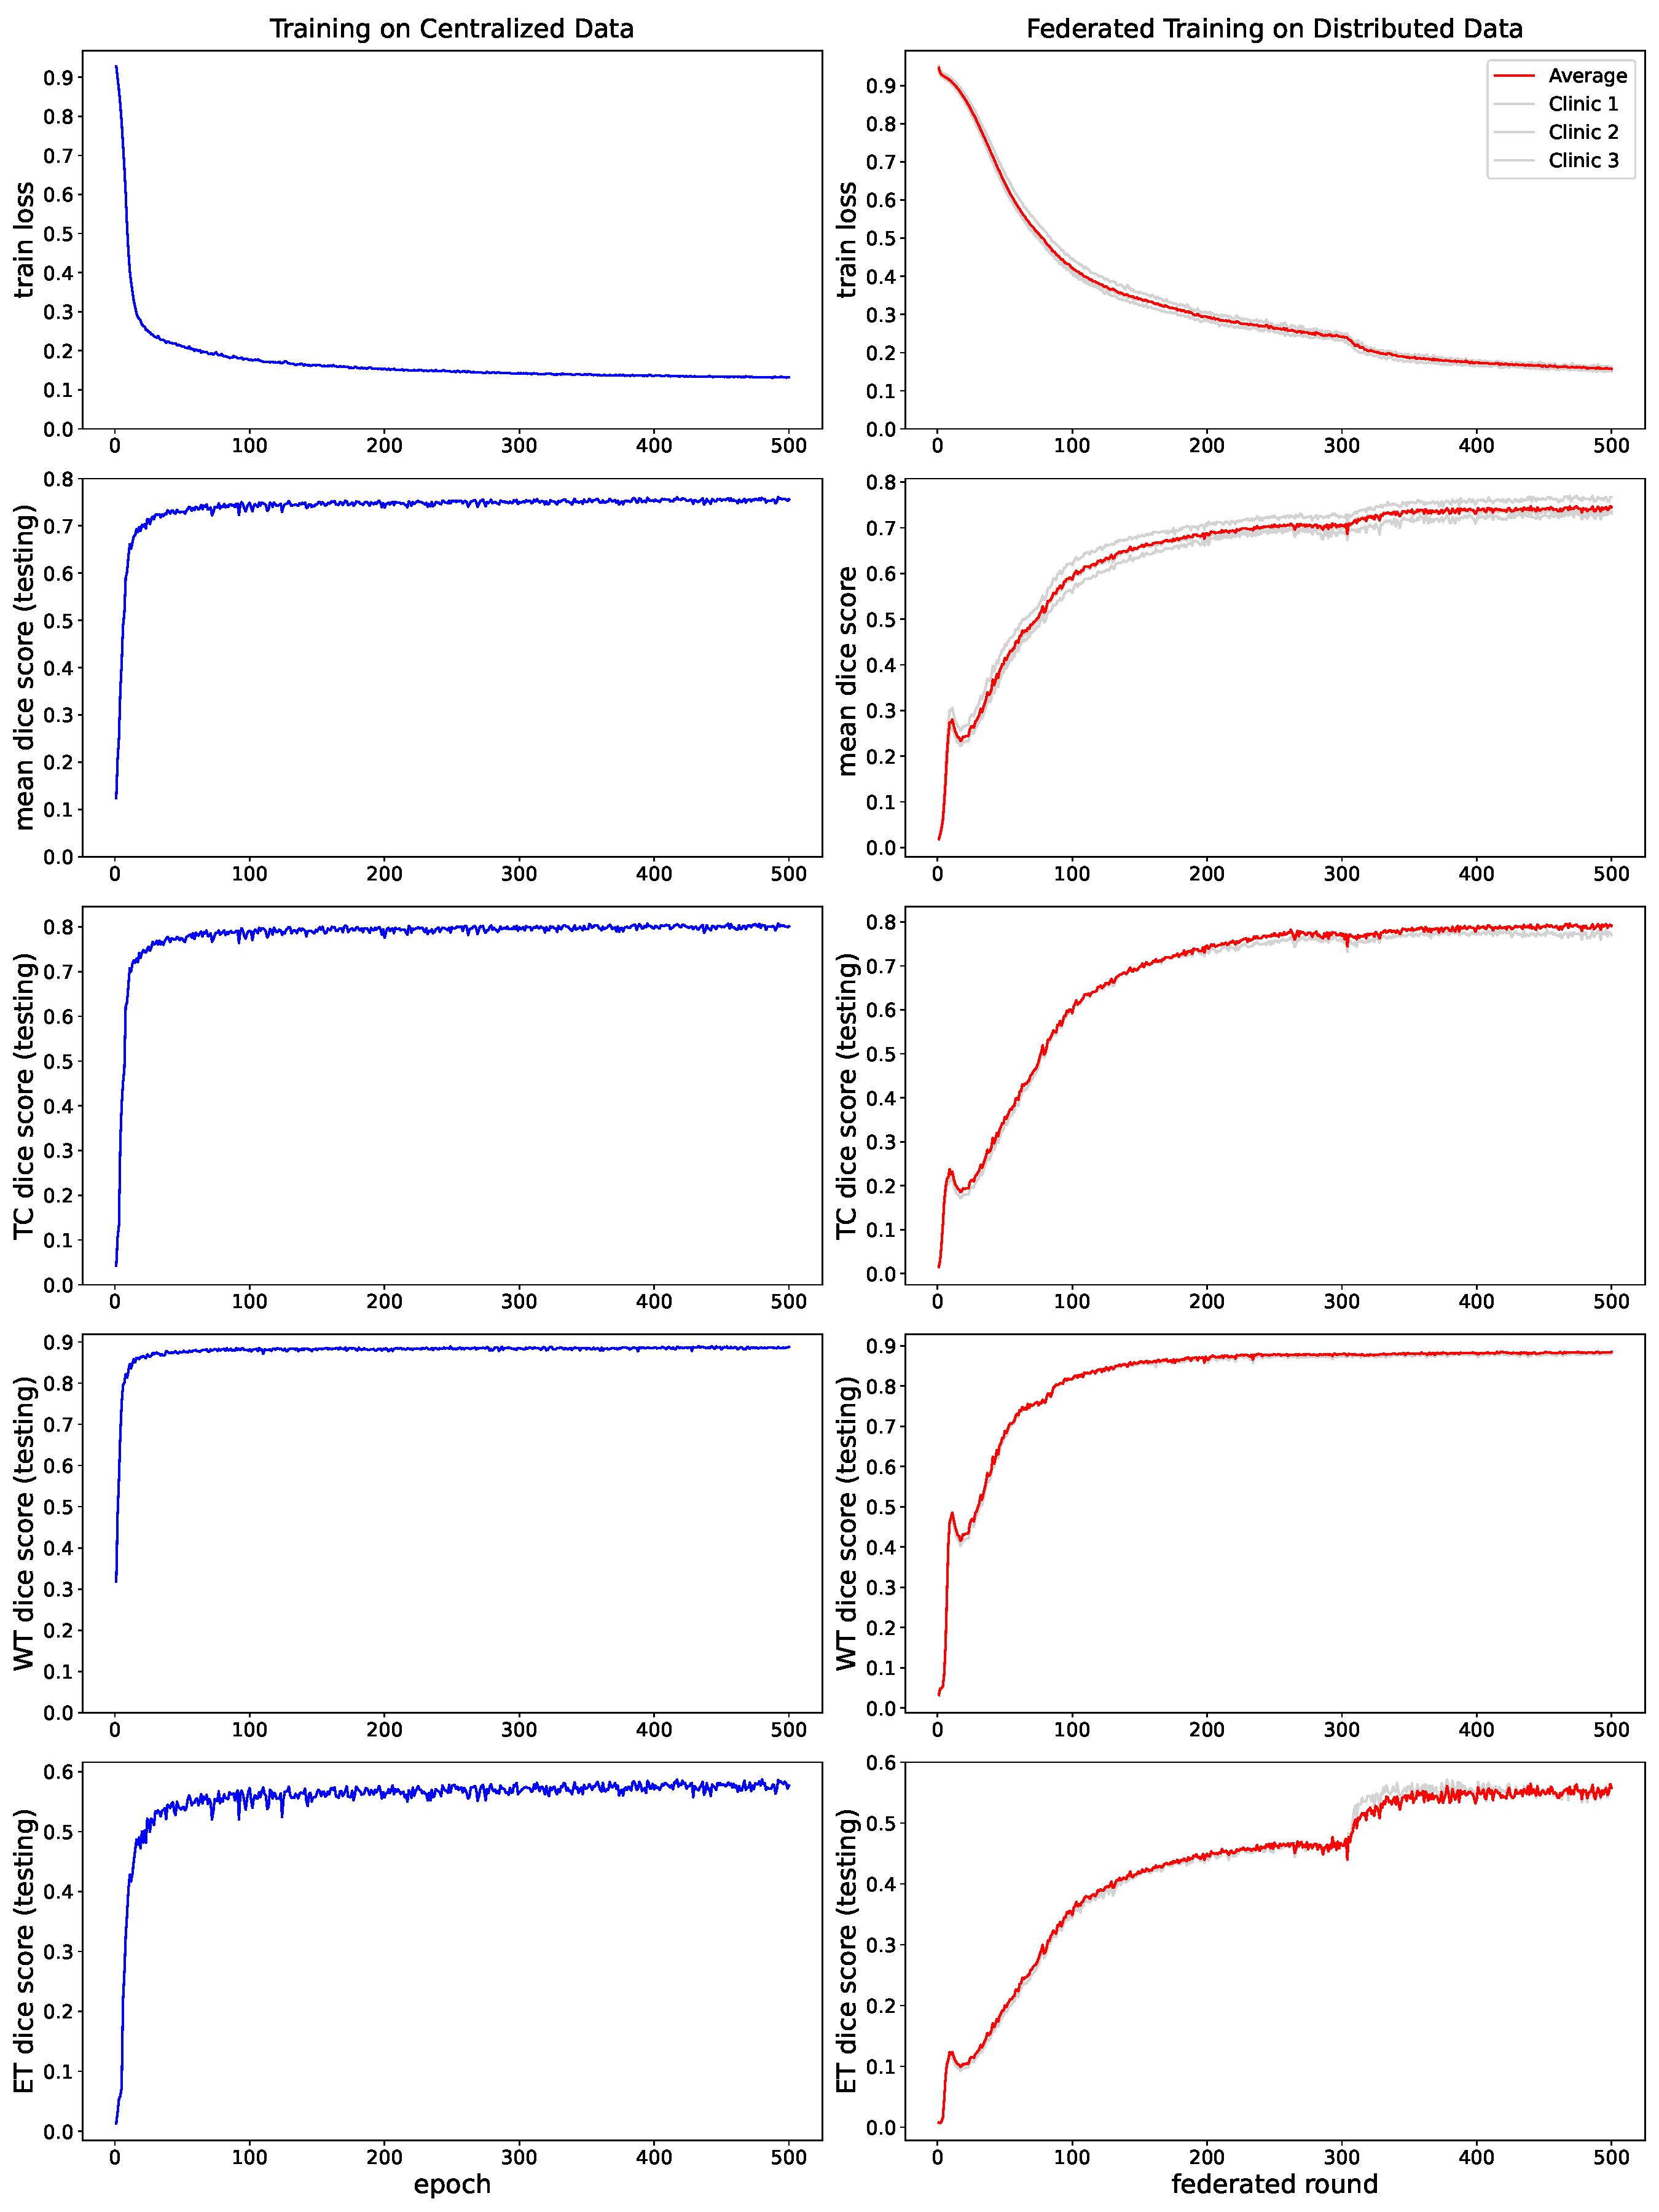
\includegraphics[width=1.0\textwidth]{1_Figures/BraTSexperiment_all.pdf}}
    \caption[Training loss and dice scores of the conducted BraTS experiment]{Training loss and testing performance of models trained on centralized data (blue) and in a federated scenario across three participating clinics (red). Curves are displayed for the three segmentation masks tumor core (TC), whole tumor (WT), enhancing tumor (ET) and their mean scores.}
    \label{fig:BraTSplots}
\end{figure}

 
 \section{Discussion}
\label{sec:Discussion}

\subsection{Requirements \& Comparison of FL Solutions}
\label{subsec:DiscussionRequirements}

When examining the previously presented comparison (see \Cref{subsec:ResultsRequirements} on page \pageref{subsec:ResultsRequirements}) of the various FL Solutions, the following can be noted.
% GPU 
Apart from PySyft all FL solutions support GPU. This also applies to the current version of the PriMIA extension, which has been adapted for the field of medical image data.
% PACS & DICOM
Both, NVIDIA Clara Federated and JIP Federated provide an adapter for the clinical PACS, which is particularly advantageous in the field of medical image processing, while all others do not. The same applies to the support of the DICOM format, which is equally essential.
Note that PriMIA extends PySyft in such a way that it supports DICOM while PySyft itself does not.
% Information
Except for PySyft and PaddleFL all solutions come with extensive information. While PySyft does not yet provide a complete and detailed documentation, the resources regarding PaddleFL are not fully provided in English language. In addition, the community of PaddleFL communicates mainly in Chinese.

% privacy things - Lack of privacy mechanism on JIP federated
When comparing the privacy mechanisms, a weakness of JIP Federated becomes apparent. All other solutions support at least one of the considered mechanisms, whereas JIP Federated has not implemented any mechanism yet.
Note that TFF does not natively come with Differential Privacy. However, it can be seamlessly added by using TensorFlow Privacy\footnote{\url{https://github.com/tensorflow/privacy}}, which is completely interoperable with TFF.
While the implementation of such mechanisms is beyond the scope of this work, it is foreseeable that this will be one of the next steps in further development. % hier angebracht?
Until then, this is an obvious disadvantage of JIP Federated.

% Platform solutions
NVIDIA Clara Federated and JIP Federated are both extensive platform solutions with features for the healthcare environment, and in particular for working with medical images.
% Distinction between NVIDIA Clara and JIP Federated
The differences between the two solutions are the following. While the codebase of NIVDIA Clara Federated is not publicly available, JIP Federated is fully open-source. This allows developers to extend the solution according to their needs, to understand the functionalities, and therefore trust the solution.
From our perspective, all this can be seen as advantageous.
Further, NVIDIA Clara Federated provides the privacy mechanisms Differential Privacy and Homomorphic Encryption, which is a major advantage compared to JIP Federated, which does not support such mechanisms yet.

% Limitation
Please note that this categorization was done to the best of our knowledge and based on the available information. As mentioned before, it was not always easy to identify the relevant details in the given information.





\subsection{Implementation of PySyft Integration \& JIP Federated}
\label{subsec:DiscussionImplementation}
% ### PySyft Integration ###
% (Docker) container integration
As the PySyft components are available as containers, the integration into the JIP is seamlessly possible. This also applies to the integration as container-based operators into a DAG.
Additionally, the usage of the PySyft-Notebook is not mandatory. The software library can also be installed independently of the provided container and used within a python script, for example.

% flexibilität der JIP durch PySyft Integration gezeigt
% Old: PySyft and therefore its integration into the JIP comes with the drawback of long computing times as shown in the experiments. However, the 
The integration of PySyft clearly shows the advantages of the JIP. 
It highlights the flexibility and expandability of the platform, not only for PySyft but also for other potential solutions and frameworks. We showed that due to the open codebase, it is possible to combine other FL solutions with the JIP. In particular, solutions that are provided as containers can be deployed seamlessly in the JIP's Kubernetes cluster.

% ### JIP Federated ####
For JIP Federated, the key component to orchestrate the workflows within and across the central instance and the participants is Airflow.
% re-using operators
Because Airflow operators are the essential components for the workflow logic, they should be as generic and reusable as possible to minimize the development effort for a new experiment. We have managed to implement all operators, except the actual experiment operators, in such a way that they are completely transferable as they are. Therefore, a data scientist who wants to conduct his experiment in the JIP only needs to transfer his code into the two containers for model aggregation and model training on the participants. We see this as advantageous in terms of development effort.

% Drawback of number of operator being used 
A drawback of the JIP federated implementation is the large number of operators needed for the individual tasks.
Especially, the scheduling DAG on the central instance requires numerous operators. This is necessary to implement the different steps of the workflow logic but brings an unfortunate side effect: Due to the dependencies between the individual tasks, the operators can only work in parallel to a minor extent.
% reasoning
Since each operator needs time to be started up and shut down again, even tasks that are actually fast require more time.
% idle time disadvantage relative
This idle time accumulates and adds up to the actual processing time. This disadvantage is reduced in its impact for experiments in which the actual training on the participants takes a larger share of the overall workflow time than the process on the central instance.
This is particularly evident in the results of the runtime experiments listed in \Cref{tab:RuntimeExp}.
The implementations' runtime for model training does differ only by a few minutes when using MNIST data. In contrast, PySyft requires more than twice as long as JIP Federated for the more complex task on the pneumonia data.

% Different data handling % Transformations
Further, there is a difference between the PySyft Integration and JIP Federated in terms of data handling and pre-processing.
With PySyft the random transformations are applied to the images only once. The data-providing operator then serves the pre-processed images in this form for the whole training via the PySyft node on the CPU. In contrast, JIP Federated applies new random transformations in each federated round. This results in a higher variability within the images used for training,
which then becomes apparent during model training and final testing.






\subsection{Experiments}
\label{subsec:DiscussionExperiments}

% ### Runtime Comparison ###
For the runtime experiments on the MNIST and pneumonia datasets,
% similarity of behavior
the shape of the training curves and the performance of the resulting models are comparable. The models trained with JIP Federated perform only slighly better according to accuracy and ROC-AUC. Thus, the implementations lead to similar training behavior, and the runtime can be compared with each other.
% different learning curve
The reason for the slightly different training curves on the pneumonia images can be found in the differences in the implementations mentioned before.
Applying the image transformations only once leads to a smaller variance in the training data of the PySyft experiment and, therefore, to a lower training loss. However, the resulting model generalizes slightly poorer, which explains the weaker test performance of the model trained with PySyft.
% spikes
The noticeable peaks during training on the pneumonia data might be due to outliers or poor data labelling.

% Runtime
Although the runtime experiments themselves are relatively basic, both solutions require a rather long time.
However, the difference of more than seven hours when training on the pneumonia dataset demonstrates the shortcomings regarding the computing efficiency of PySyft. The comparatively long training time has already been noted by the developers and explained by the implemented privacy mechanisms \citep{Ryffel2018ALearning}.
JIP Federated also requires rather a long time for the experiments, which can be explained by the already mentioned large number of required Airflow operators.



Examining the training behavior of the federated segmentation experiment,
% Federated 
we find that the curves are very similar for all three participants. The apparent reason for this is that the BraTS data was distributed randomly and not according to its origin or some criteria that influence the imaging, such as the used hardware.
Further, the curves of the dice scores have notable buckles at two points, which also can be identified in the shape of the loss curve during training. The first occurs after about ten federated rounds and the second after 300. The buckles can also be seen in the ET and TC curves, in the latter in particular the second one is very significant. The first buckle occurs strongly in all dice score curves.
Furthermore, the curve of the dice score for the ET segmentation mask converges later and less stable compared to the curves for the TC and WT segmentation masks.

% Comparison to centralized
When comparing the federated experiment with the centralized setting, some differences can be observed as well.
% buckles
First, the buckles seen during the federated training do not occur in the traditional setting of training on centralized data. We suspect that this could be due to the chosen \textit{optimizer state treatment}, but have not conducted experiments with other treatment options.
% slower convergence
Further, the model converges more slowly in a federated setting. One reason for this is probably the aggregation of the models: a simple average of model parameters cannot adequately combine the knowledge learned at the different sites. This is the usual trade-off FL faces: the convergence could be accelerated by performing fewer local training steps (moving closer to mini-batch gradient descent), but that would increase the communication frequency.
% "Noise"
What can also be noted is that in both experiments, the convergence on the TC and ET segmentation masks is less stable than on the WT segmentation masks.

% final performance
Although the convergence is slower, the model trained with FL achieves a mean dice score of 0.745 after 500 epochs. This is equivalent to 98.58 \% of the performance by the model trained on centralized data (mean dice score of 0.7554). Thus, it can be said that the federated trained model converges slower, but nearly reaches the upper performance baseline.
% Performance
In general, it can be noted that it is more difficult for the models to segment the ET region. Compared to segmenting the TC and WT regions, the dice score is significantly lower. This, of course, also considerably lowers the overall performance measured as mean dice score.
In both, the federated and centralized experiment, the highest values are obtained on the WT segmentation masks.
Note also that we did not perform any hyperparameter tuning for FL and just adopted the parameters that were provided in the MONAI tutorial\footnote{\url{https://github.com/Project-MONAI/tutorials/blob/master/3d\_segmentation/brats\_segmentation\_3d.ipynb}; commit hash: d340613cea8b0f10b780694c636c1d7ff8f7658d}, which was developed on centralized data.

% centralized (last testing (val)):    0.7554029747843742
% federated (last testing (val) avg):  0.7446803177396456
% compared:                         98.58053814948381

 
 \section{Conclusion \& Outlook}
\label{sec:ConclusionOutlook}

\subsection{Conclusion}
\label{subsec:Conclusion}
% intro
In order to use deep learning models in clinics, they must be robust and generalize sufficiently. One way to achieve this is to train these models on very large datasets. However, annotated image data in the healthcare domain is rare and expensive---and is subject to privacy aspects.
Federated learning is a promising approach to address these challenges. But first, technical solutions are needed to enable the application of federated learning in the healthcare environment.

% We compared exisiting federated learning solutions with regrad to what is needed bring federated learnign into medical institutions. Thus, we provide an overview of solutions in the 
% there is not yet one solution that meets all requirements, but promising solutions are emerging.

% Solution comparison
We showed which federated learning solutions exist and what is needed to bring federated learning into medical institutions. There is not yet one solution that meets all requirements, but many promising projects could be identified.
% on federated learning and also its application within the healthcare environment.
The platform solutions NVIDIA Clara Train and JIP Federated, the latter of which is presented within this article, provide features that are advantageous for the application in the healthcare environment, in particular for the usage of medical images.

We demonstrated that the Joint Imaging Platform is a promising solution, either in combination with an existing federated learning framework or as a stand-alone solution itself.
% Integration
With the seamless integration of PySyft, the high flexibility of the platform was demonstrated, so the possibility to combine other solutions with the Joint Imaging Platform's infrastructure and the resulting benefits are given.
% JIP Federated
Further, we designed a JIP-only federated learning solution---JIP Federated.
By using JIP Federated for the segmentation of gliomas in brain MRI scans, we demonstrated that it is a capable federated learning solution for complex medical task. Its implementation is highly flexible, easy to apply on other federated learning experiments, and brings further advantages through its platform features.
Thus, we provide a comprehensive open-source solution to conduct real-world federated learning in the domain of medical image computing.

% ### Outlook ###
% Advantage: Established & Trusted
The Joint Imaging Platform is an established and trusted tool in the healthcare community and is already being used in a multitude of German clinics and beyond.
As proved by the experiments, JIP Federated can be a solution to make federated learning real-world.
% real-world experiment with lots of data from 
Future work should focus on using JIP Federated for experiments across  geographically distributed clinics on large datasets that cannot be shared directly.
% Adding additional privacy mechanisms and layer between the communication of JIP instances
A further aspect needs to be the extension of the Joint Imaging Platform to provide privacy mechanisms such as Differential Privacy, Homomorphic Encryption, and Secure Multi-Party Computing as additional security layers for the communication between instances.
% Motivation zur Anwendung in der Praxis tatsächlich ohen den Zugang zu den ganzen Daten.
With this work on federated learning with the Joint Imaging Platform, we also hope to give an incentive for further federated experiments using JIP Federated.
% We want to encourage the further development and long-term use of JIP Federated in practice and for large-scale studies.

\subsection{Outlook}
\label{subsec:Outlook}

Medical image analysis has come a long way from rule-based systems and handcrafted features for early computer vision to modern techniques. Nowadays, deep learning is the technology of choice in computer vision and therefore also for medical images. In recent time, it has proved its capabilities and potential on a multitude of tasks in the domain of medical images. Deep learning is currently and will be in the future the technology for processing and analyzing medical images. However, its full potential can only be unlocked if the appropriate volume of data is available to train such deep architectures.

% federated learning
Federated learning provides a solution to overcome the challenge of not having a sufficient amount of data. If the gap between simulation and real application can be closed by developing comprehensive technical solutions, enormous volumes of data will be available for usage. All around the world, respective data is collected on a daily basis, but until now it has not been available for traditional machine learning settings, also for reasons of patients privacy and regulations. The data would be accessible and usable by means of technical solutions for federated learning across geographically distributed institutions.

% results
Using this data would result in among others two consequences.
The developed models can achieve significantly higher performance on numerous tasks, which is in particular important in a critical field like healthcare where life and death can be at stake.
Further, these models will be able to generalize better because of their extensive knowledge base. That is, they are more capable to adapt to previously unseen samples which do not fall into the distribution of the samples used for training. 
All of this would be possible, because systems are available that have gained experience from the data of millions of patients and the knowledge of numerous medical experts who labeled the data.
% improve health-care service
Such comprehensive systems can contribute to improve healthcare, individualize patient treatment, and to better understand or even cure severe and rare diseases.
% remote areas 
Further, models with high performance and the ability to generalize sufficiently could even be used as a form of decision support in regions of the world with poor or hardly any advanced healthcare services.

% final
Certainly, many things remain to be done to bring the technical solutions to the point where federated learning projects truly go across medical institutions, but first steps are being taken. The healthcare sector remains very sensitive, highly regulated and also political, but there are more than just a few researches and practitioners who see federated learning as the future of digital health \citep{Rieke2020TheLearning}.


% BACKUP

%Further, one can imagine that models with high performance and the ability to generalize sufficiently can actually be developed by using the data volumes that will be available with real-world federated learning. The resulting solutions and services could even be used in regions of the world with only poor or hardly any healthcare services.
 
% % % % % % % % % % % % % ANHANG% % % % % % % % % % % % % % % % 

%\appendix 
%\section{Appendix}
\label{sec:Appendix}


% ### APPENDIX PART A ###




\begin{sidewaystable}
%\begin{table*}[h!]
  \centering
  \begin{tabular}{cccccccc}
    Reference & Scenario & FL Solution & Participants & Computing Plan & Algorithm & Task \\
    \hline \\[-1.5ex]
    \cite{Xu2020ADiagnosis}                             & real-world & custom solution          & 4             & FedAvg                    & 3D-Densenet       & Classification \\
    \cite{Balachandar2020AccountingImaging}             & simulated  & -                        & 4             & Sequential                & GoogleLeNet       & Classification \\
    \cite{Wang2020AutomatedLearning}                    & real-world & NVIDIA Clara Federated   & 2             & FedAvg                    & C2FNAS            & Segmentation \\
    \cite{Remedios2020DistributedSegmentation}          & real-world & custom solution          & 2             & Sequential                & U-Net             & Segmentation  \\
    \cite{Remedios2019DistributedInjury}                & real-world & custom solution          & 2             & Sequential                & CNN (Incept.)     & Segmentation  \\
    \cite{Chang2018DistributedImaging}                  & simulated  & -                        & 4             & Sequential \& Ensembling  & ResNet34          & Classification \\
    \cite{Kaissis2021End-to-endImaging}                 & synthetic  & PriMIA (based on PySyft) & 3             & FedAvg                    & ResNet18          & Classification  \\
    \cite{Dou2021FederatedStudy}                        & synthetic  & custom solution          & 3             & FedAvg                    & CNN               & Segmentation \\
    \cite{Roth2020FederatedImplementation}              & real-world & NVIDIA Clara Federated   & 7             & FedAvg                    & DenseNet-121      & Classification \\
    \cite{Feki2021FederatedImages}                      & simulated  & -                        & 4             & FedAvg                    & VGG16 \& ResNet50 & Classification \\    
    \cite{Sarma2021FederatedSharing}                    & real-world & NVIDIA Clara Federated   & 3             & FedAvg                    & 3D AH Net         & Segmentation \\
    \cite{Sheller2020FederatedData}                     & simulated  & -                        & 10            & FedAvg \& Sequential      & U-Net             & Segmentation \\
    \cite{Baheti2020FederatedNodules}                   & simulated  & -                        & 3             & FedAvg                    & V-Net             & Classification \\    
    \cite{Yang2021FederatedJapan}                       & synthetic  & NVIDIA Clara Federated   & 3             & FedAvg                    & 3D U-Net          & Segmentation \\  
    \cite{Sheller2019Multi-institutionalSegmentation}   & simulated  & -                        & 4, 6, 8, 32   & FedAvg                    & U-Net             & Segmentation \\
    \cite{Li2019Privacy-preservingSegmentation}         & synthetic  & NVIDIA Clara Federated   & 13            & FedAvg                    & CNN               & Segmentation \\
    \cite{Andreux2020SiloedDatasets}                    & simulated  & -                        & 2, 5          & FedAvg                    & CNN               & Segmentation \\
    \cite{Yan2020Variation-AwareData}                   & simulated  & -                        & 2, 4, 8       & FedAvg                    & CNN               & Classification \\
    \cite{Lee2021FederatedEnvironment}                  & real-world & PySyft                   & 6             & FedAvg                    & multiple          & Classification \\
    \cite{Flores2021FederatedPatients}\rlap{*}          & real-world & NVIDIA Clara Federated   & 20            & FedAvg                    & ResNet34          & Classification \\
  \end{tabular}
  \caption{Complete list of articles applying FL using medical images in a real-world, synthetic, or simulated scenario (*Preprint)}
  \label{tab:LitSearchFull}
%\end{table*}
\end{sidewaystable}



\newpage
% ### APPENDIX PART B ###
\subsection{Detailed parameters and training information for the conducted experiments}
\label{apdx:B}

\Cref{tab:TrainingParams} provides an overview of the used training parameters for the three conducted experiments.
Further, the model architectures used for the experiments as well as the applied image transformations are explained in the following.

% transposed table


% ### MNIST - Experiment Details ###
The MNIST experiment was derived from PyTorch example\footnote{https://github.com/pytorch/examples/blob/master/mnist/main.py; commit hash: 0f0c9131ca5c79d1332dce1f4c06fe942fbdc665}. The model architecture consist of two convolutional layers followed by max pooling and a dropout layer. The two subsequent fully connected layers are separated by a second dropout layer.
Except for normalization, no transformations were applied to the images.


% ### Pneumonia - Experiment Details ###
As in the article of \cite{Kaissis2021End-to-endImaging}, ResNet18 \cite{He2016DeepRecognition} was chosen as model architecture for the experiment on the pneumonia data. Please note that due to the mentioned limitations of PySyft, Stochastic Gradient Descent (SGD) and not Adam was used as optimizer.
The following transformations were applied to the images.
Image resizing to $256 \times 256$,
random horizontal flipping,
random vertical flipping,
and image normalization.


% ### BraTS - Experiment Details ###
The configuration for the segmentation experiment using the brain MRI scans is based on the corresponding MONAI tutorial\footnote{\url{https://github.com/Project-MONAI/tutorials/blob/master/3d\_segmentation/brats\_segmentation\_3d.ipynb}; commit hash: d340613cea8b0f10b780694c636c1d7ff8f7658d}.
The U-Net architecture was set up with a channel sequence of ($16, 32, 64, 128, 256$) and convolution strides of size two. The number of residual units was set to two.
% channels=(16, 32, 64, 128, 256),
% strides=(2, 2, 2, 2),
% num_res_units=2,
The following transformation were applied on the brain scans.
Random vertical flipping,
random spacial cropping ($\textrm{with roi\_size} =  128 \times 128 \times 64$),
intensity normalization,
random intensity shifting,
random intensity scaling.
Note that apart from the parameters listed in \Cref{tab:TrainingParams}, the Adam optimizer \cite{Kingma2014Adam:Optimization} was used with its PyTorch default values. 

% % % % % % % % % % % % % LITERATUR% % % % % % % % % % % % % % %
%\phantomsection
\renewcommand\bibname{References}
\bibliographystyle{apalike}
%\bibliography{References.bib}
\bibliography{references.bib}
\end{document}
